\documentclass[10pt]{beamer}
\usepackage[english]{babel}
\usepackage[utf8]{inputenc}
\usepackage[T1]{fontenc}
\usepackage{helvet}

%-------------------------------------------------------
% INFORMATION IN THE TITLE PAGE
%-------------------------------------------------------

\newcommand{\cstitle}{\textbf{Bioinformatics}}
\subtitle[]{DNA structure and replication}
\newcommand{\cscourseCode}{1005155}
\newcommand{\csauthor}{MSc. Vicente Machaca Arceda}
\institute[UNSA]{Universidad Nacional de San Agustín de Arequipa}
\newcommand{\csemail}{vmachacaa@unsa.edu.pe}
\newcommand{\instituteabr}{UNSA}
\newcommand{\nameUp}{ICC Fase 1}
\date{\today}
\title[\cscourseCode]{\cstitle}
\author{\csauthor}
%%%%%%%%%%%%%%%%%

%-------------------------------------------------------
% CHOOSE THE THEME
%-------------------------------------------------------
\def\mycmd{0} % CS THEME
%\def\mycmd{1} % MYTHEME
%-------------------------------------------------------

\if\mycmd1
\usetheme[]{Feather}
\newcommand{\chref}[2]{	\href{#1}{{\usebeamercolor[bg]{Feather}#2}} }
\else
\usepackage{csformat}
\fi

\newcommand{\1}{
	\setbeamertemplate{background}{
		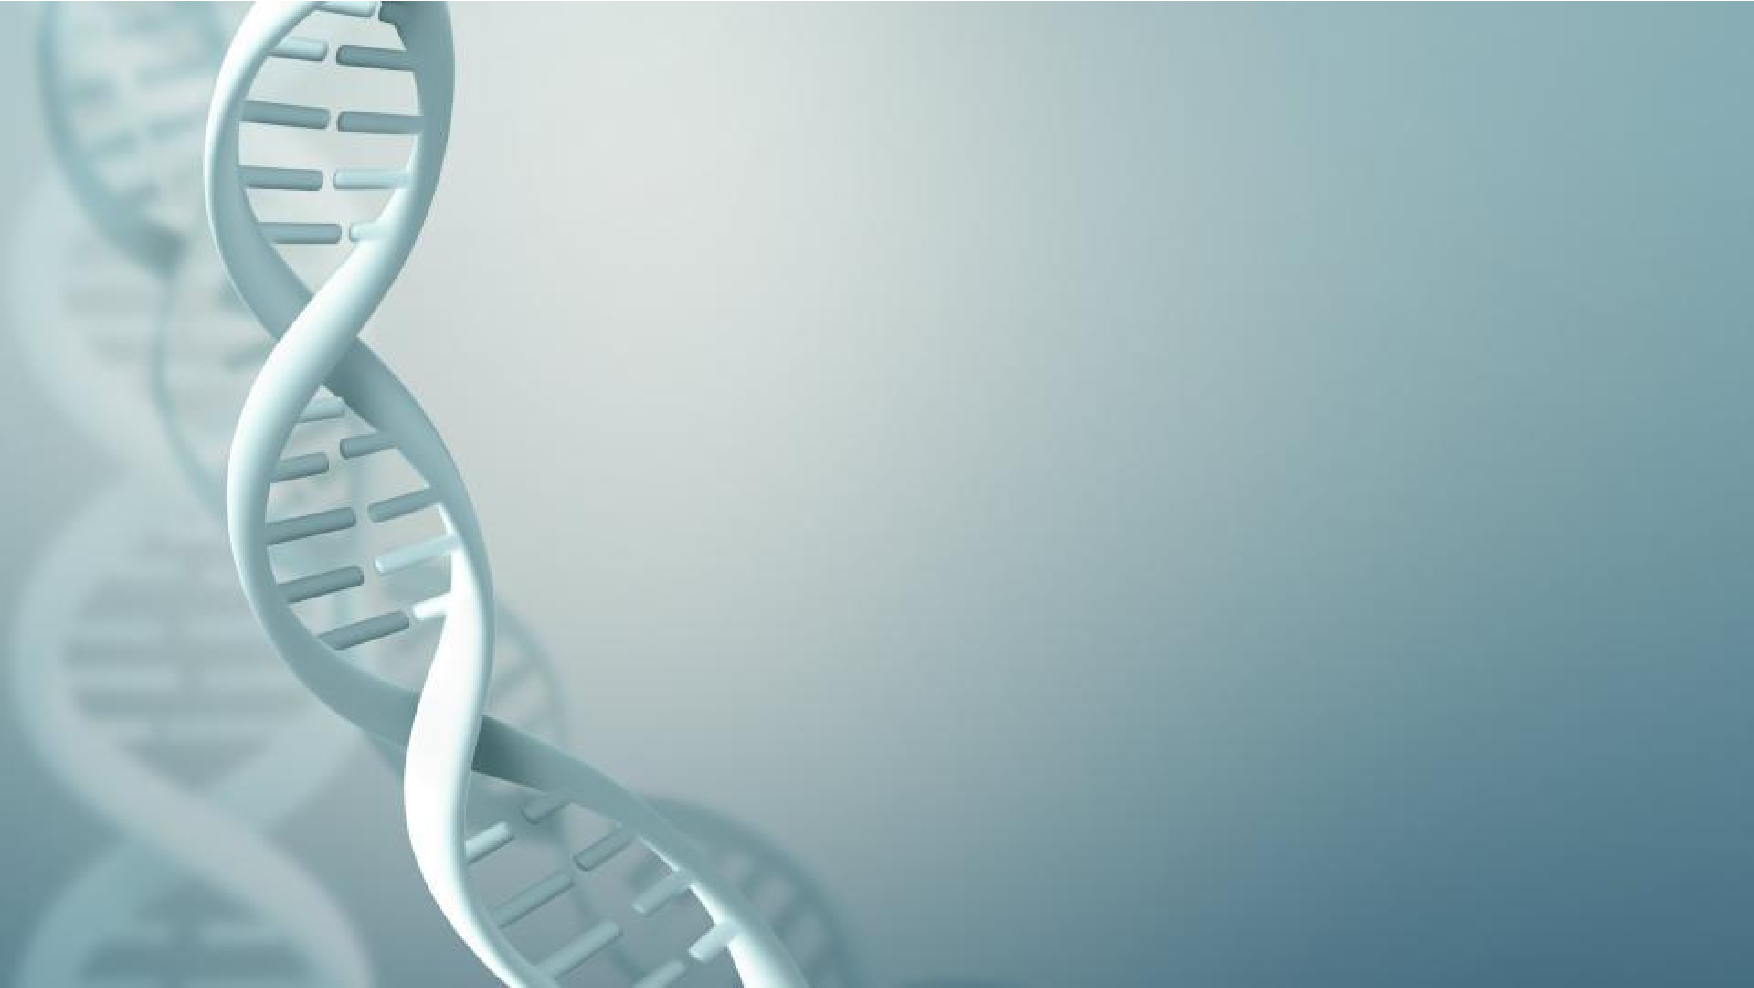
\includegraphics[width=\paperwidth,height=\paperheight]{img/1}
		\tikz[overlay] \fill[fill opacity=0.75,fill=white] (0,0) rectangle (-\paperwidth,\paperheight);
	}
}



%-------------------------------------------------------
% THE BODY OF THE PRESENTATION
%-------------------------------------------------------

\begin{document}
	
	
	\AtBeginSection[]
	{
		\begin{frame}
			\frametitle{Table of Contents}
			\tableofcontents[currentsection]
		\end{frame}
	}
	
	
%-------------------------------------------------------
% THE TITLEPAGE
%-------------------------------------------------------

\if\mycmd1 % MY THEME
\1{
	\begin{frame}[plain,noframenumbering] 
		\titlepage 
	\end{frame}}
	
	\else % CS THEME
	\maketitle
\fi

%-------------------------------------------------------
%-------------------------------------------------------
\begin{frame}{Table of Contents}
\tableofcontents
\end{frame}
%-------------------------------------------------------
%-------------------------------------------------------

%%%%%%%%%%%%%%%%%%%%%%%%%%%%%%%%%%%%%%%%%%%%%%%%%%%%%%%%%%%%%%%%%%%%%%%%%%%%%%%%%%%%%%%%%%%%%%%%%%%%%%%%%%%%%%%%
%%%%%%%%%%%%%%%%%%%%%%%%%%%%%%%%%%%%%%%%%%%%%%%%%%%%%%%%%%%%%%%%%%%%%%%%%%%%%%%%%%%%%%%%%%%%%%%%%%%%%%%%%%%%%%%%
%%%%%%%%%%%%%%%%%%%%%%%%%%%%%%%%%%%%%%%%%%%%%%%%%%%%%%%%%%%%%%%%%%%%%%%%%%%%%%%%%%%%%%%%%%%%%%%%%%%%%%%%%%%%%%%%
\section{Introduction}
%%%%%%%%%%%%%%%%%%%%%%%%%%%%%%%%%%%%%%%%%%%%%%%%%%%%%%%%%%%%%%%%%%%%%%%%%%%%%%%%%%%%%%%%%%%%%%%%%%%%%%%%%%%%%%%%
%%%%%%%%%%%%%%%%%%%%%%%%%%%%%%%%%%%%%%%%%%%%%%%%%%%%%%%%%%%%%%%%%%%%%%%%%%%%%%%%%%%%%%%%%%%%%%%%%%%%%%%%%%%%%%%%
%%%%%%%%%%%%%%%%%%%%%%%%%%%%%%%%%%%%%%%%%%%%%%%%%%%%%%%%%%%%%%%%%%%%%%%%%%%%%%%%%%%%%%%%%%%%%%%%%%%%%%%%%%%%%%%%




%%%%%%%%%%%%%%%%%%%%%%%%%%%%%%%%%%%%%%%%%%%%%%%%%%%%%%%%%%%%%%%%%%%%%%%%%%%%%%%%%%%%%%%%%%%%%%%%%%%%%%%%%%%%%%%%
%%%%%%%%%%%%%%%%%%%%%%%%%%%%%%%%%%%%%%%%%%%%%%%%%%%%%%%%%%%%%%%%%%%%%%%%%%%%%%%%%%%%%%%%%%%%%%%%%%%%%%%%%%%%%%%%
%%%%%%%%%%%%%%%%%%%%%%%%%%%%%%%%%%%%%%%%%%%%%%%%%%%%%%%%%%%%%%%%%%%%%%%%%%%%%%%%%%%%%%%%%%%%%%%%%%%%%%%%%%%%%%%%
\subsection{Objectives}
%%%%%%%%%%%%%%%%%%%%%%%%%%%%%%%%%%%%%%%%%%%%%%%%%%%%%%%%%%%%%%%%%%%%%%%%%%%%%%%%%%%%%%%%%%%%%%%%%%%%%%%%%%%%%%%%
%%%%%%%%%%%%%%%%%%%%%%%%%%%%%%%%%%%%%%%%%%%%%%%%%%%%%%%%%%%%%%%%%%%%%%%%%%%%%%%%%%%%%%%%%%%%%%%%%%%%%%%%%%%%%%%%
%%%%%%%%%%%%%%%%%%%%%%%%%%%%%%%%%%%%%%%%%%%%%%%%%%%%%%%%%%%%%%%%%%%%%%%%%%%%%%%%%%%%%%%%%%%%%%%%%%%%%%%%%%%%%%%%

%-------------------------------------------------------
%-------------------------------------------------------
\begin{frame}{Objectives}{}
\begin{itemize}
    \item<1-> Learn all chemical elements of DNA. 
    \item<2-> Understand DNA replication process.
  \end{itemize}
\end{frame}
%-------------------------------------------------------
%-------------------------------------------------------

%%%%%%%%%%%%%%%%%%%%%%%%%%%%%%%%%%%%%%%%%%%%%%%%%%%%%%%%%%%%%%%%%%%%%%%%%%%%%%%%%%%%%%%%%%%%%%%%%%%%%%%%%%%%%%%%
%%%%%%%%%%%%%%%%%%%%%%%%%%%%%%%%%%%%%%%%%%%%%%%%%%%%%%%%%%%%%%%%%%%%%%%%%%%%%%%%%%%%%%%%%%%%%%%%%%%%%%%%%%%%%%%%
%%%%%%%%%%%%%%%%%%%%%%%%%%%%%%%%%%%%%%%%%%%%%%%%%%%%%%%%%%%%%%%%%%%%%%%%%%%%%%%%%%%%%%%%%%%%%%%%%%%%%%%%%%%%%%%%
\section{DNA structure and replication}
%%%%%%%%%%%%%%%%%%%%%%%%%%%%%%%%%%%%%%%%%%%%%%%%%%%%%%%%%%%%%%%%%%%%%%%%%%%%%%%%%%%%%%%%%%%%%%%%%%%%%%%%%%%%%%%%
%%%%%%%%%%%%%%%%%%%%%%%%%%%%%%%%%%%%%%%%%%%%%%%%%%%%%%%%%%%%%%%%%%%%%%%%%%%%%%%%%%%%%%%%%%%%%%%%%%%%%%%%%%%%%%%%
%%%%%%%%%%%%%%%%%%%%%%%%%%%%%%%%%%%%%%%%%%%%%%%%%%%%%%%%%%%%%%%%%%%%%%%%%%%%%%%%%%%%%%%%%%%%%%%%%%%%%%%%%%%%%%%%




%%%%%%%%%%%%%%%%%%%%%%%%%%%%%%%%%%%%%%%%%%%%%%%%%%%%%%%%%%%%%%%%%%%%%%%%%%%%%%%%%%%%%%%%%%%%%%%%%%%%%%%%%%%%%%%%
%%%%%%%%%%%%%%%%%%%%%%%%%%%%%%%%%%%%%%%%%%%%%%%%%%%%%%%%%%%%%%%%%%%%%%%%%%%%%%%%%%%%%%%%%%%%%%%%%%%%%%%%%%%%%%%%
%%%%%%%%%%%%%%%%%%%%%%%%%%%%%%%%%%%%%%%%%%%%%%%%%%%%%%%%%%%%%%%%%%%%%%%%%%%%%%%%%%%%%%%%%%%%%%%%%%%%%%%%%%%%%%%%
\subsection{DNA structure}
%%%%%%%%%%%%%%%%%%%%%%%%%%%%%%%%%%%%%%%%%%%%%%%%%%%%%%%%%%%%%%%%%%%%%%%%%%%%%%%%%%%%%%%%%%%%%%%%%%%%%%%%%%%%%%%%
%%%%%%%%%%%%%%%%%%%%%%%%%%%%%%%%%%%%%%%%%%%%%%%%%%%%%%%%%%%%%%%%%%%%%%%%%%%%%%%%%%%%%%%%%%%%%%%%%%%%%%%%%%%%%%%%
%%%%%%%%%%%%%%%%%%%%%%%%%%%%%%%%%%%%%%%%%%%%%%%%%%%%%%%%%%%%%%%%%%%%%%%%%%%%%%%%%%%%%%%%%%%%%%%%%%%%%%%%%%%%%%%%



%-------------------------------------------------------
%-------------------------------------------------------
\begin{frame}{DNA structure}{Overview}

\begin{block}{}
The following content is extracted from the video \href{https://www.youtube.com/watch?v=o_-6JXLYS-k}{\textbf{The structure of DNA}} \cite{yourgenome2020}.
\end{block}

\end{frame}
%-------------------------------------------------------
%-------------------------------------------------------

%-------------------------------------------------------
%-------------------------------------------------------
\begin{frame}{DNA structure}{Overview}
	\begin{figure}[]
		\centering
		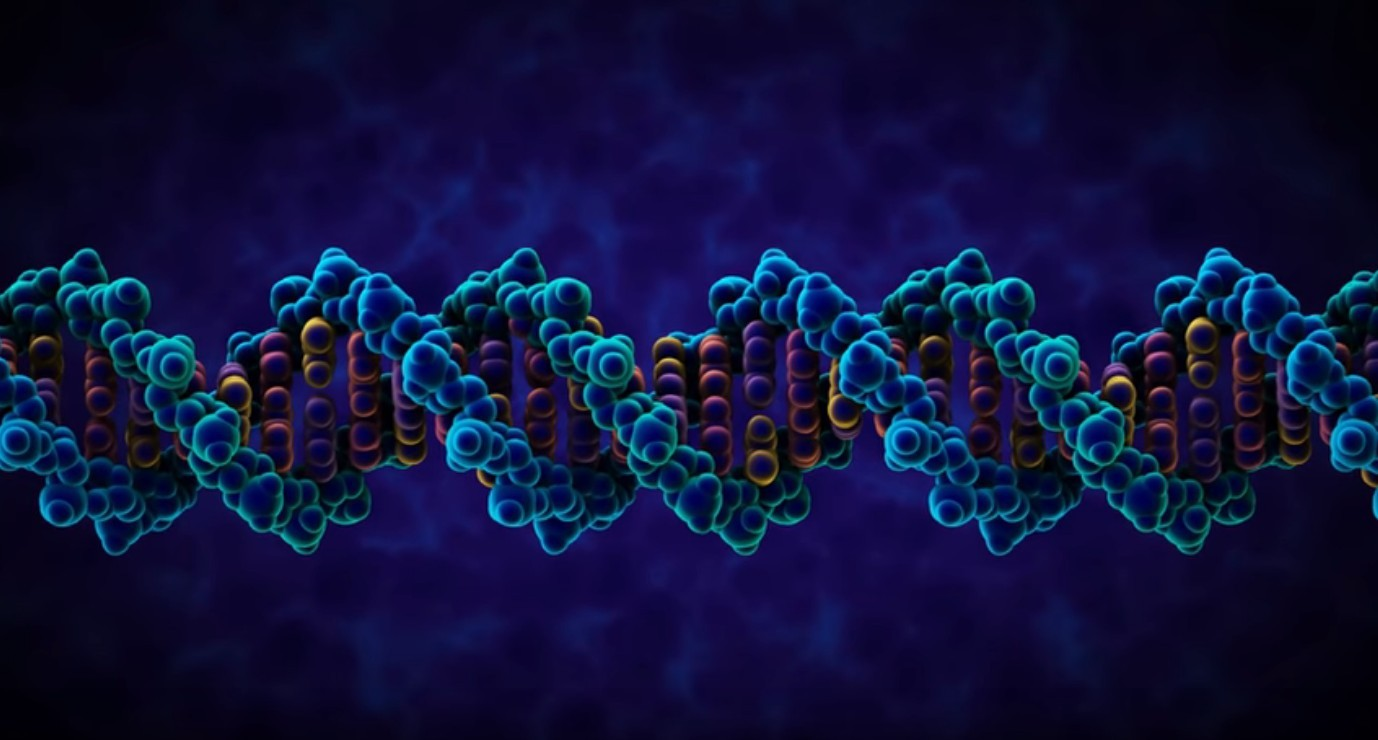
\includegraphics[width=\textwidth,height=0.7\textheight,keepaspectratio]{img/introduction/dna1.jpg}
		\label{img:mot2}
		\caption{DNA view}
	\end{figure}
\end{frame}
%-------------------------------------------------------
%-------------------------------------------------------

%-------------------------------------------------------
%-------------------------------------------------------
\begin{frame}{DNA structure}{Overview}
	\begin{figure}[]
		\centering
		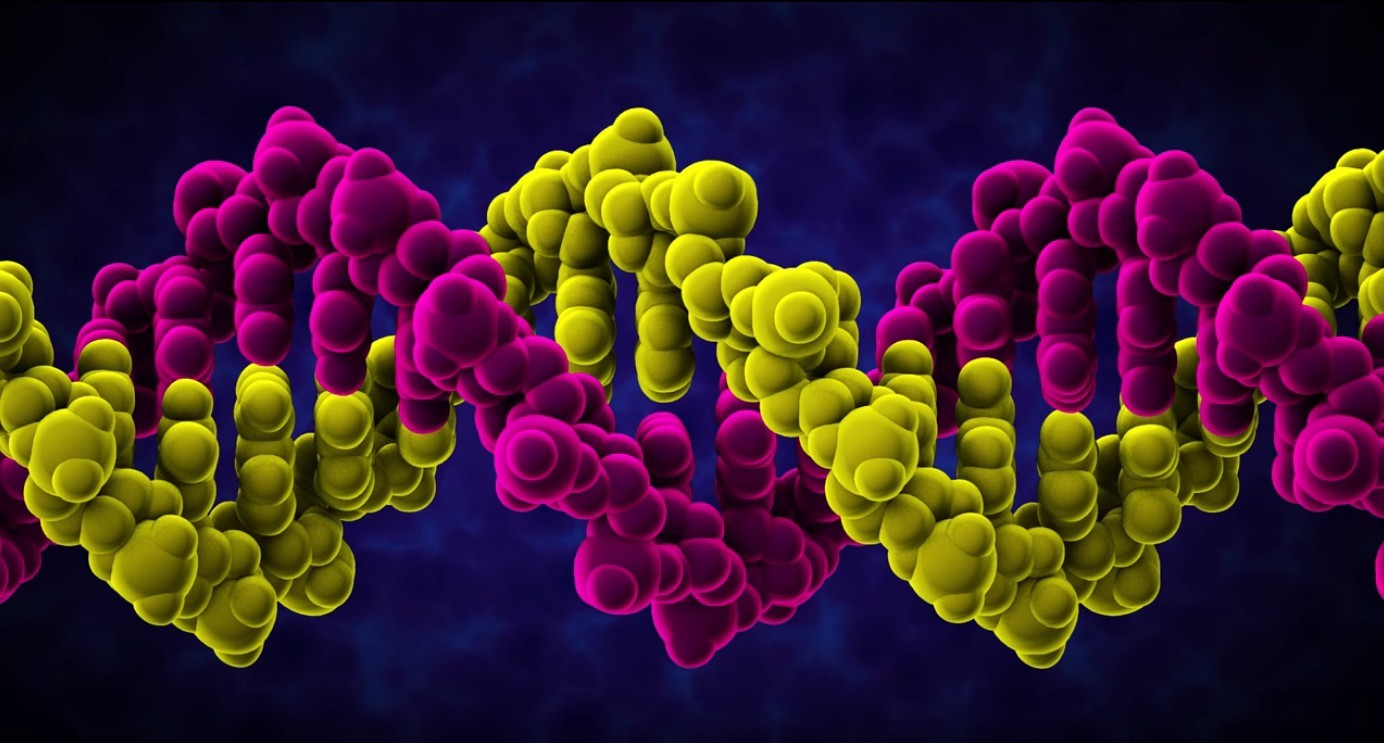
\includegraphics[width=\textwidth,height=0.7\textheight,keepaspectratio]{img/introduction/dna2.jpg}
		\label{img:mot2}
		\caption{Double strand DNA}
	\end{figure}
\end{frame}
%-------------------------------------------------------
%-------------------------------------------------------

%-------------------------------------------------------
%-------------------------------------------------------
\begin{frame}{DNA structure}{Overview}
	\begin{figure}[]
		\centering
		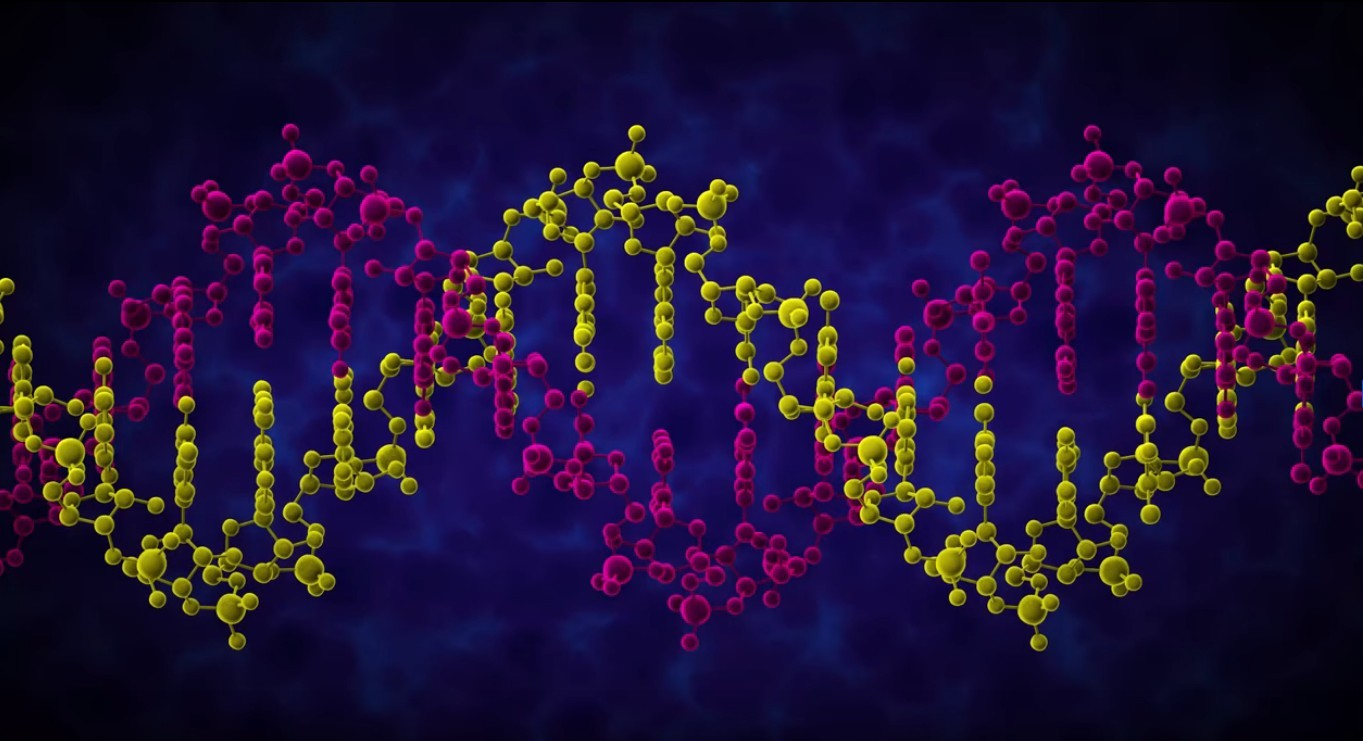
\includegraphics[width=\textwidth,height=0.7\textheight,keepaspectratio]{img/introduction/dna3.jpg}
		\label{img:mot2}
		\caption{Simplified view of DNA}
	\end{figure}
\end{frame}
%-------------------------------------------------------
%-------------------------------------------------------

%-------------------------------------------------------
%-------------------------------------------------------
\begin{frame}{DNA structure}{Overview}
	\begin{figure}[]
		\centering
		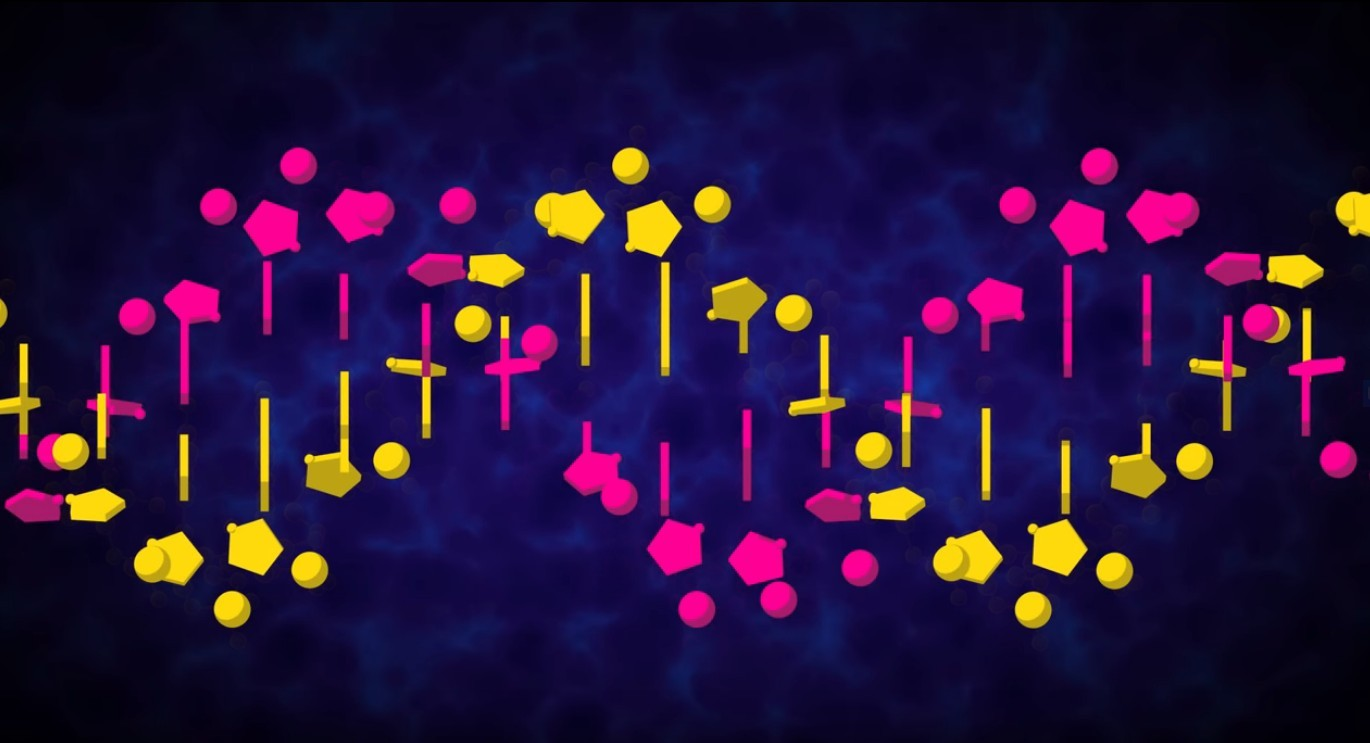
\includegraphics[width=\textwidth,height=0.7\textheight,keepaspectratio]{img/introduction/dna4.jpg}
		\label{img:mot2}
		\caption{Simplified view of DNA}
	\end{figure}
\end{frame}
%-------------------------------------------------------
%-------------------------------------------------------

%-------------------------------------------------------
%-------------------------------------------------------
\begin{frame}{DNA structure}{Overview}
	\begin{figure}[]
		\centering
		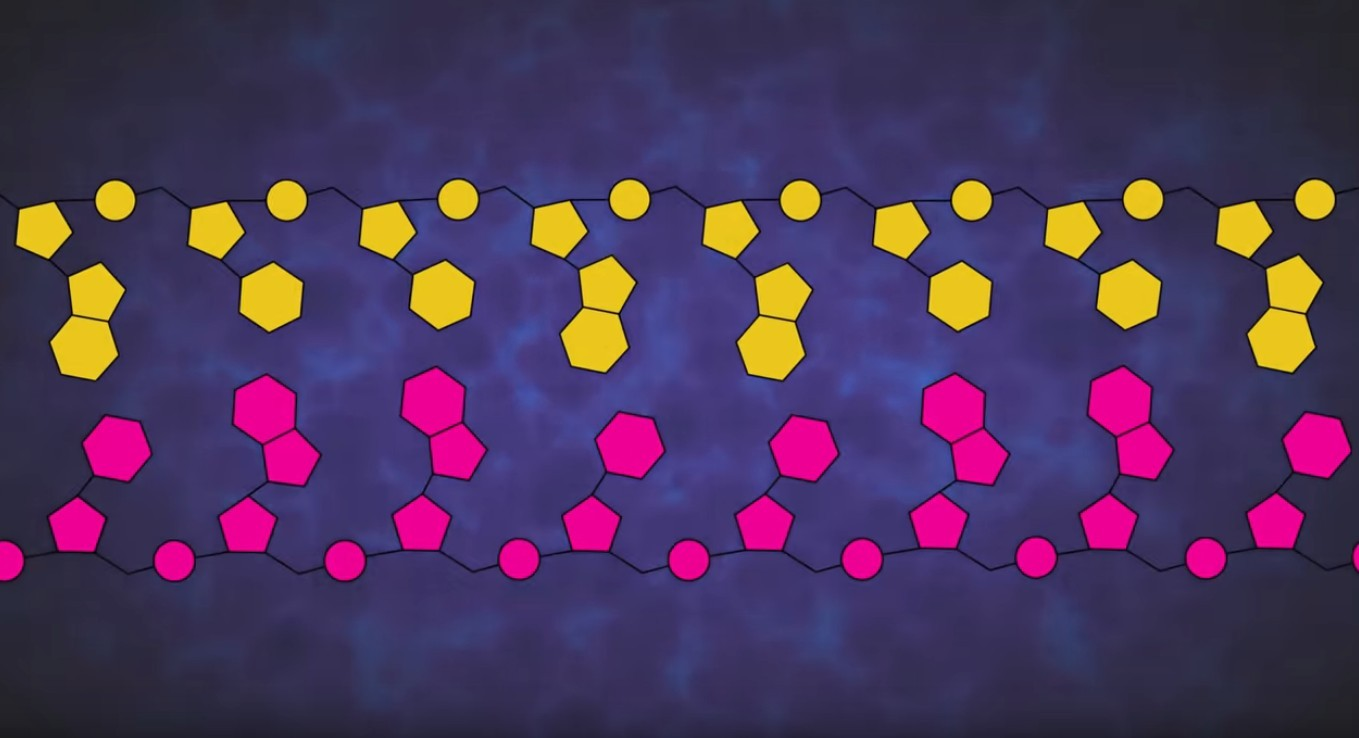
\includegraphics[width=\textwidth,height=0.7\textheight,keepaspectratio]{img/introduction/dna5.jpg}
		\label{img:mot2}
		\caption{We unwind the DNA strands.}
	\end{figure}
\end{frame}
%-------------------------------------------------------
%-------------------------------------------------------

%-------------------------------------------------------
%-------------------------------------------------------
\begin{frame}{DNA structure}{Overview}
	\begin{figure}[]
		\centering
		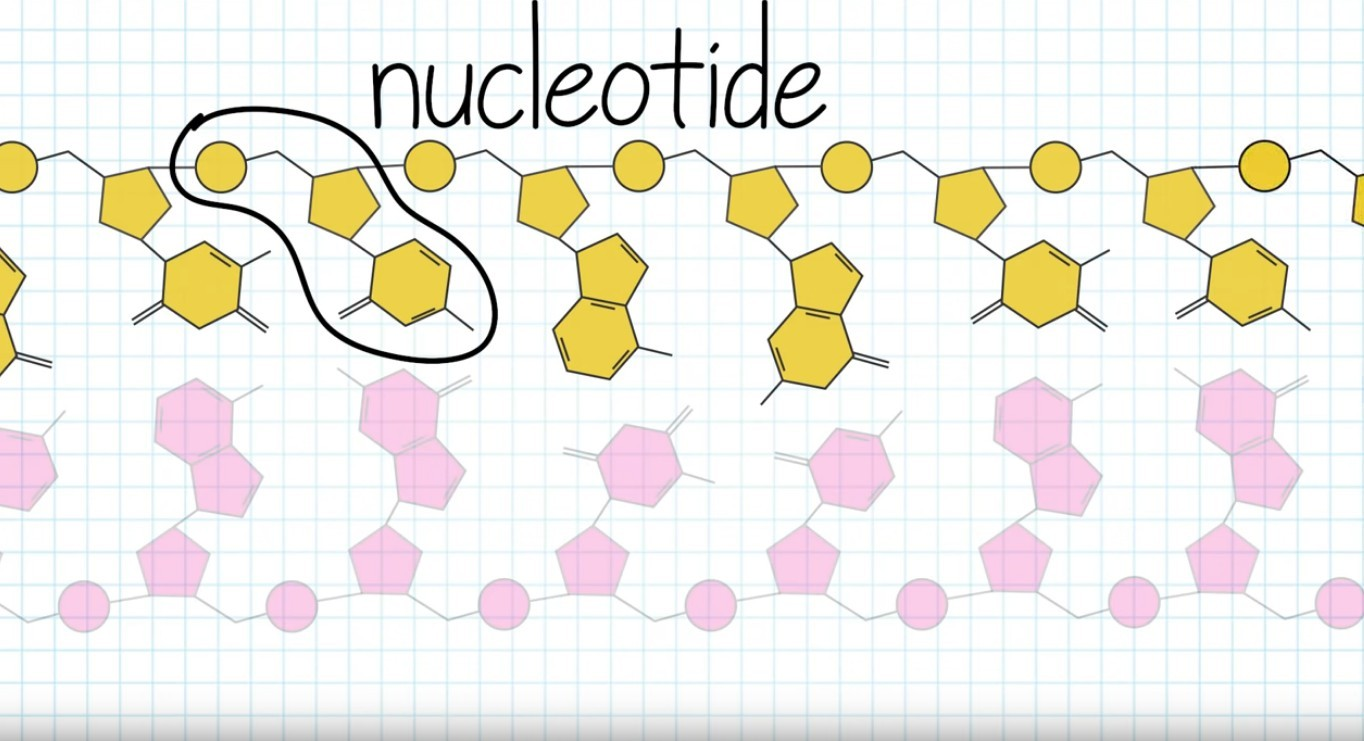
\includegraphics[width=\textwidth,height=0.7\textheight,keepaspectratio]{img/introduction/dna6.jpg}
		\label{img:mot2}
		\caption{The nucleotide in a DNA strand.}
	\end{figure}
\end{frame}
%-------------------------------------------------------
%-------------------------------------------------------

%-------------------------------------------------------
%-------------------------------------------------------
\begin{frame}{DNA structure}{Overview}
	\begin{figure}[]
		\centering
		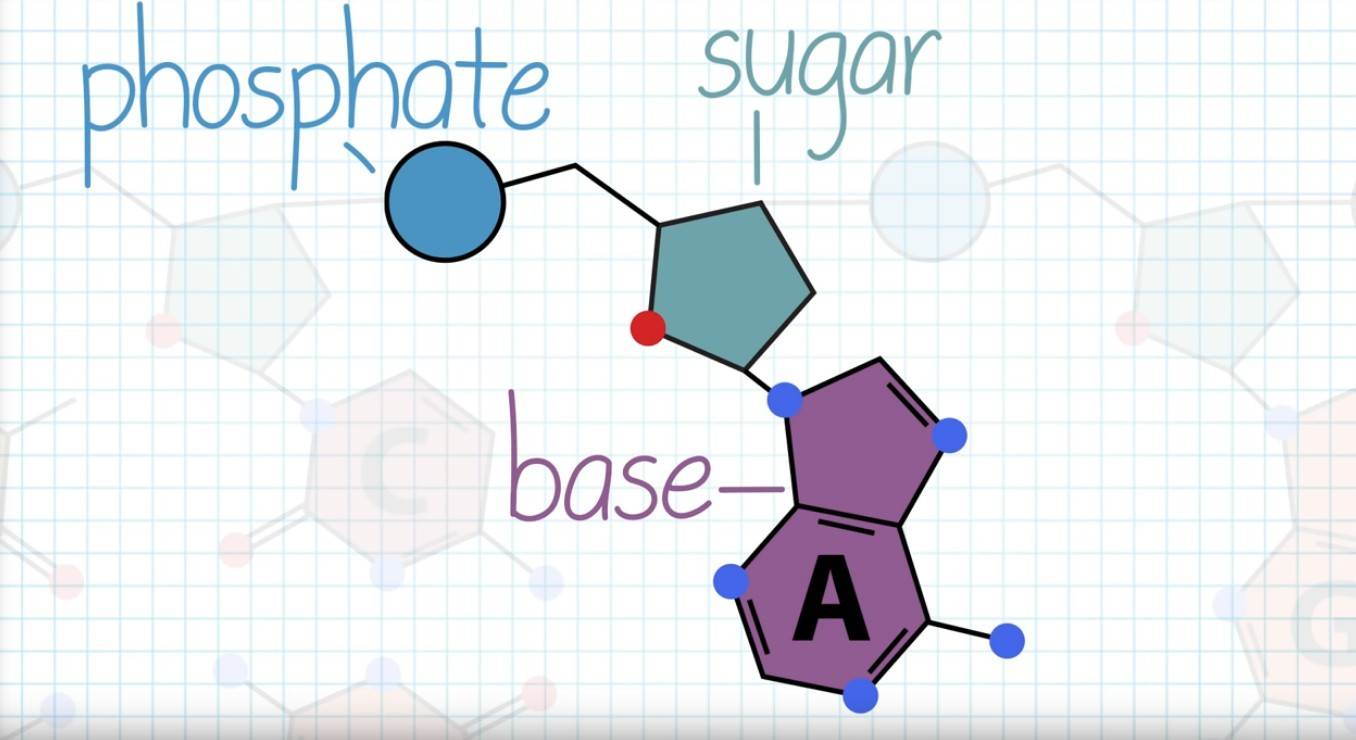
\includegraphics[width=\textwidth,height=0.7\textheight,keepaspectratio]{img/introduction/dna7.jpg}
		\label{img:mot2}
		\caption{The nucleotide have three parts: phosphate, sugar and nitrogen base.}
	\end{figure}
\end{frame}
%-------------------------------------------------------
%-------------------------------------------------------

%-------------------------------------------------------
%-------------------------------------------------------
\begin{frame}{DNA structure}{Overview}
	\begin{figure}[]
		\centering
		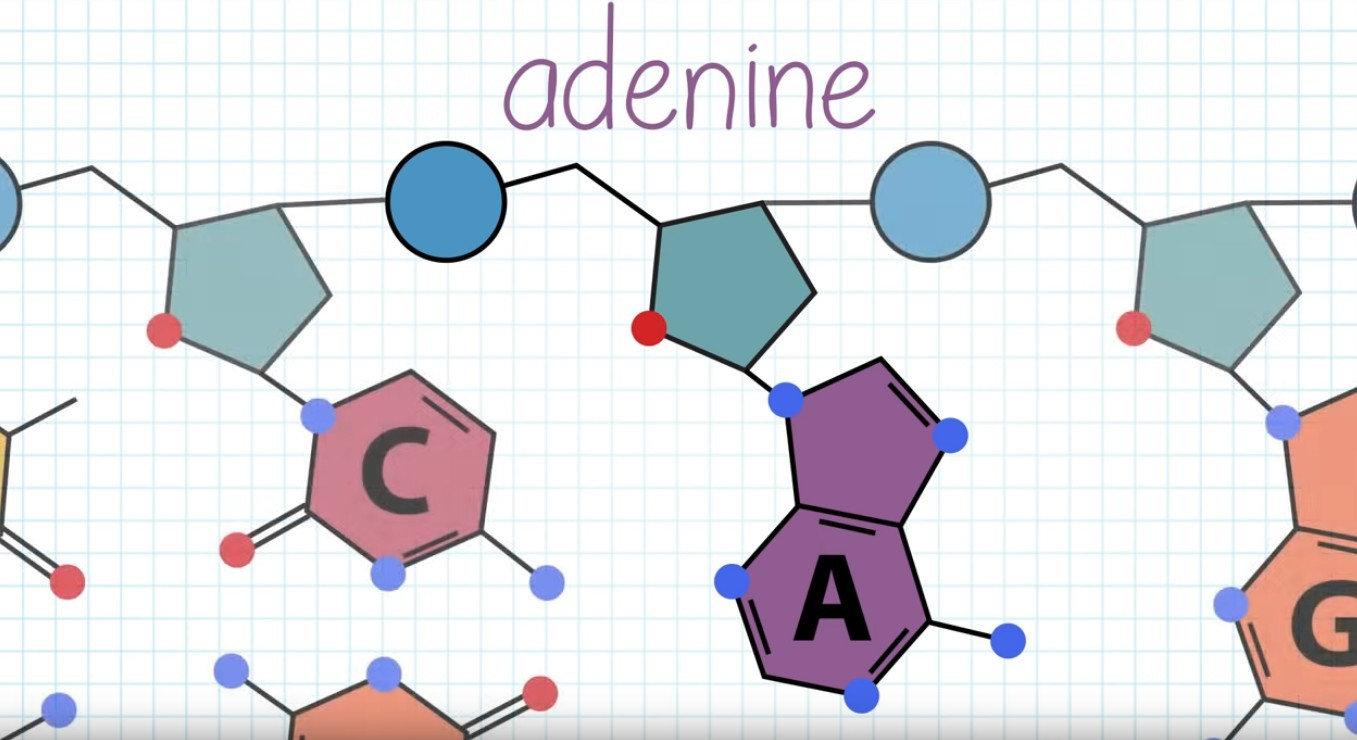
\includegraphics[width=\textwidth,height=0.7\textheight,keepaspectratio]{img/introduction/dna8.jpg}
		\label{img:mot2}
		\caption{Adenine.}
	\end{figure}
\end{frame}
%-------------------------------------------------------
%-------------------------------------------------------

%-------------------------------------------------------
%-------------------------------------------------------
\begin{frame}{DNA structure}{Overview}
	\begin{figure}[]
		\centering
		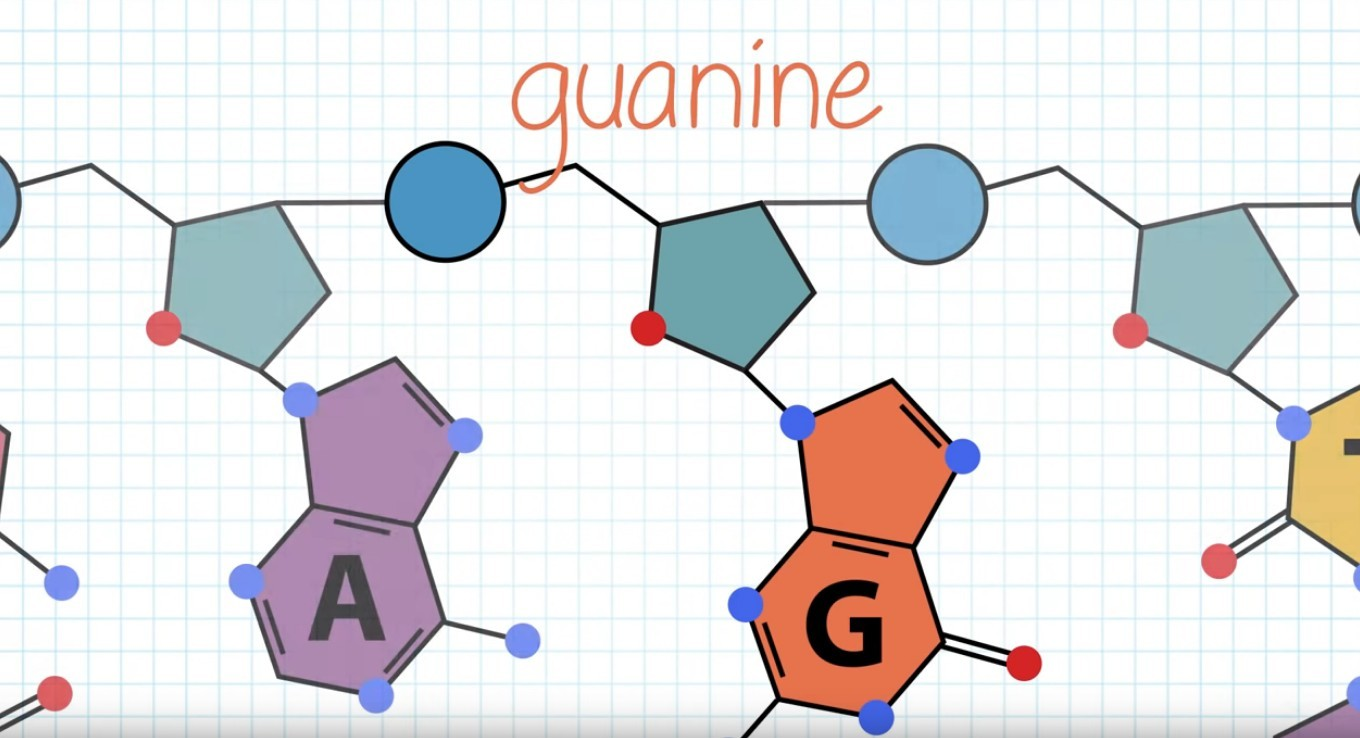
\includegraphics[width=\textwidth,height=0.7\textheight,keepaspectratio]{img/introduction/dna9.jpg}
		\label{img:mot2}
		\caption{Guanine.}
	\end{figure}
\end{frame}
%-------------------------------------------------------
%-------------------------------------------------------

%-------------------------------------------------------
%-------------------------------------------------------
\begin{frame}{DNA structure}{Overview}
	\begin{figure}[]
		\centering
		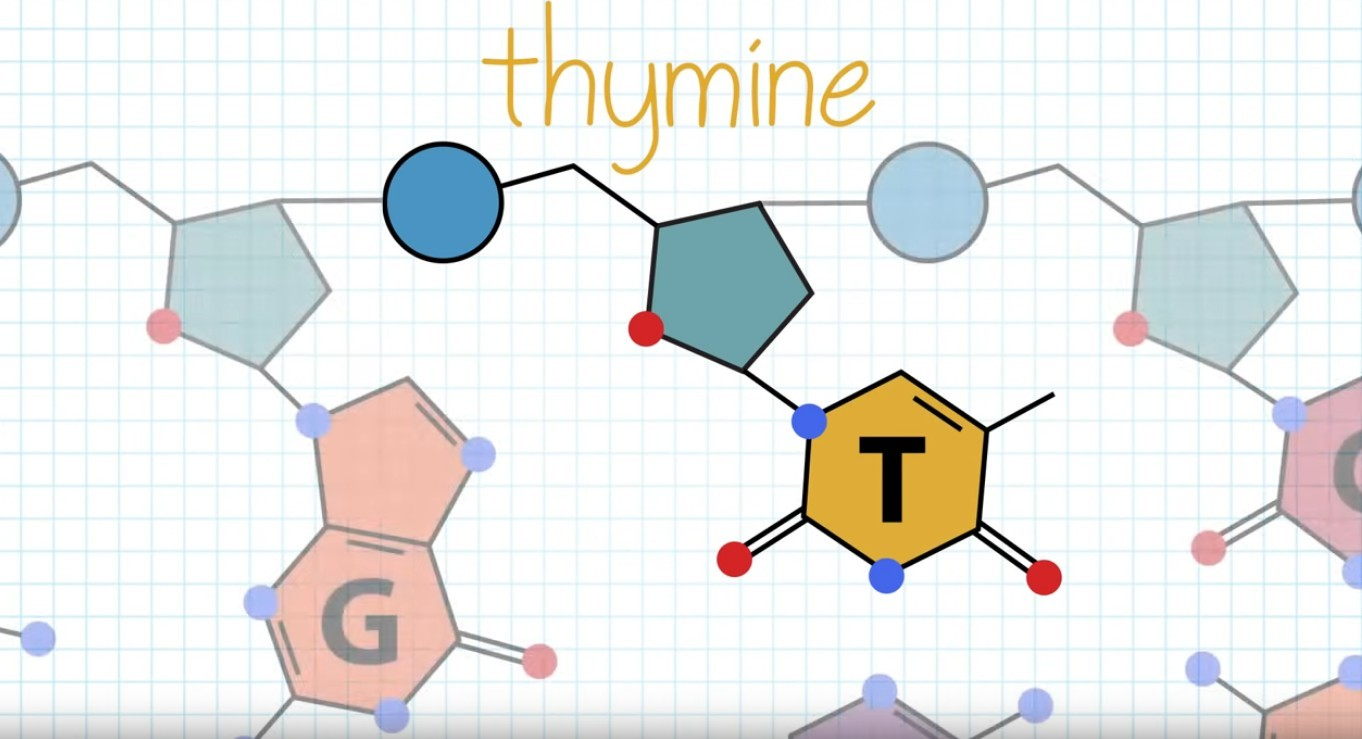
\includegraphics[width=\textwidth,height=0.7\textheight,keepaspectratio]{img/introduction/dna10.jpg}
		\label{img:mot2}
		\caption{Thymine.}
	\end{figure}
\end{frame}
%-------------------------------------------------------
%-------------------------------------------------------

%-------------------------------------------------------
%-------------------------------------------------------
\begin{frame}{DNA structure}{Overview}
	\begin{figure}[]
		\centering
		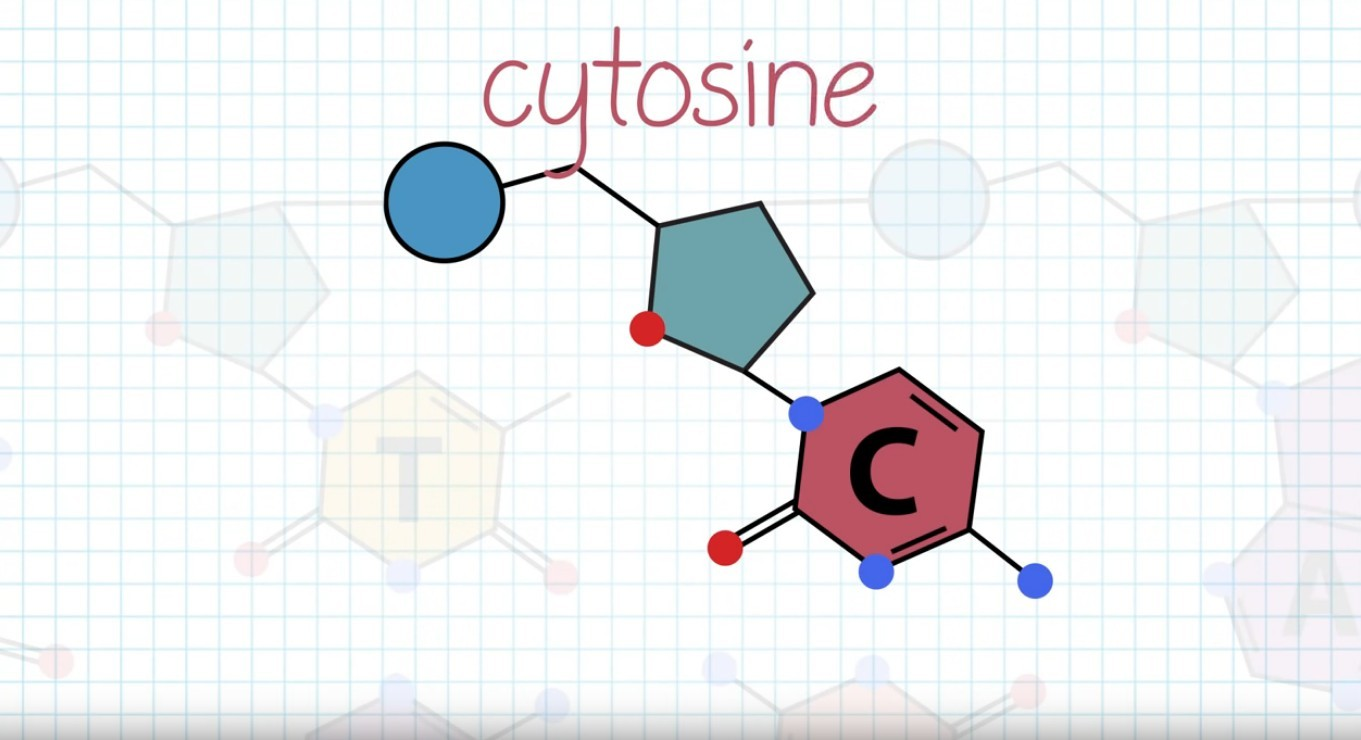
\includegraphics[width=\textwidth,height=0.7\textheight,keepaspectratio]{img/introduction/dna11.jpg}
		\label{img:mot2}
		\caption{Cytosine.}
	\end{figure}
\end{frame}
%-------------------------------------------------------
%-------------------------------------------------------

%-------------------------------------------------------
%-------------------------------------------------------
\begin{frame}{DNA structure}{Overview}
	\begin{figure}[]
		\centering
		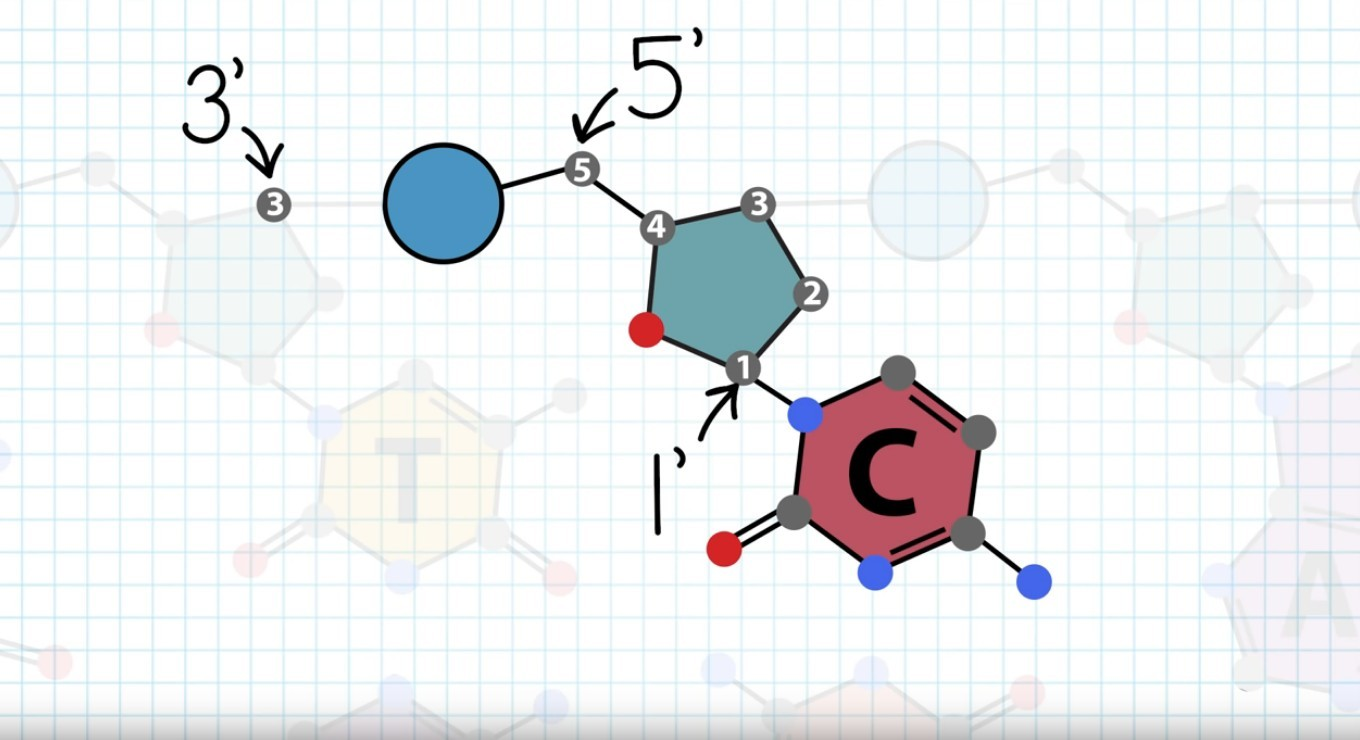
\includegraphics[width=\textwidth,height=0.7\textheight,keepaspectratio]{img/introduction/dna12.jpg}
		\label{img:mot2}
		\caption{The 1' carbon of sugar connect to the base and the 3' and 5' connect to phosphate. }
	\end{figure}
\end{frame}
%-------------------------------------------------------
%-------------------------------------------------------

%-------------------------------------------------------
%-------------------------------------------------------
\begin{frame}{DNA structure}{Overview}
	\begin{figure}[]
		\centering
		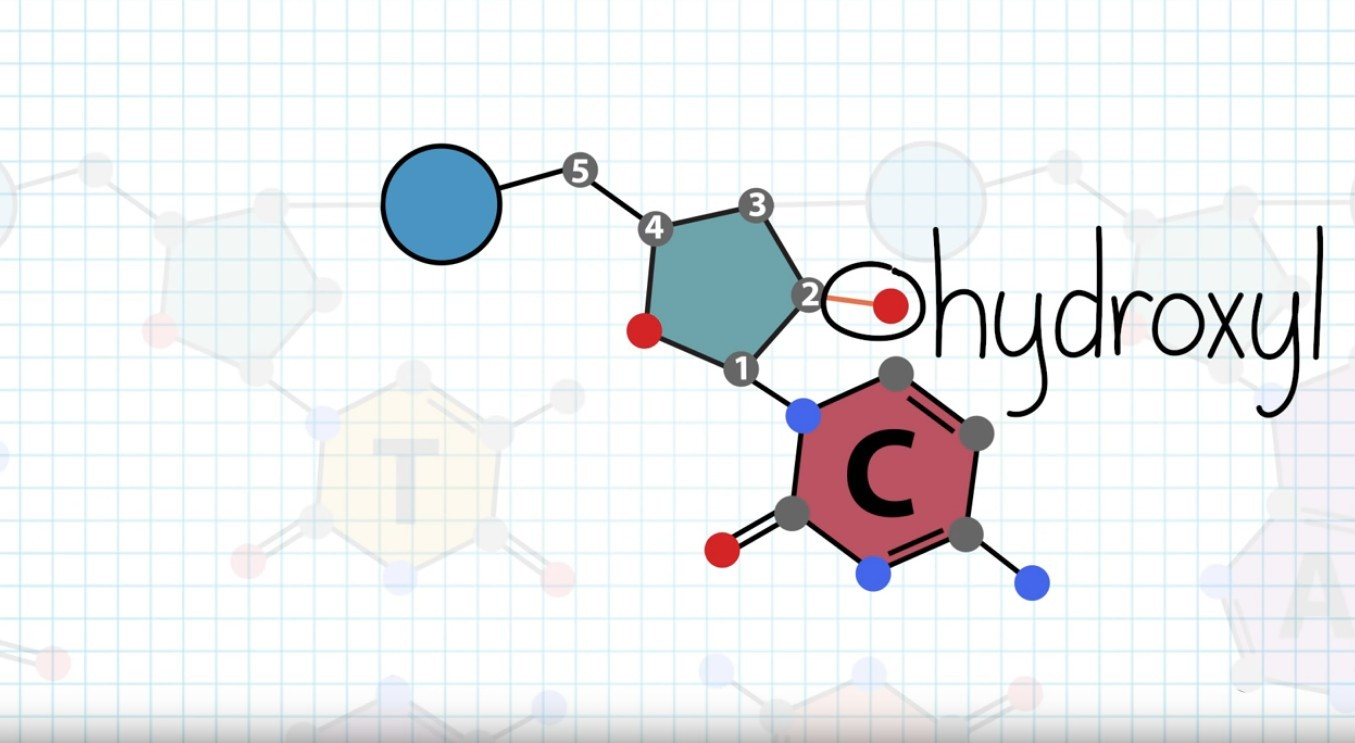
\includegraphics[width=\textwidth,height=0.7\textheight,keepaspectratio]{img/introduction/dna13.jpg}
		\label{img:mot2}
		\caption{The sugar is called deoxyribose because it is missing a hydroxyl group at her 2' carbon wich is present in ribose.}
	\end{figure}
\end{frame}
%-------------------------------------------------------
%-------------------------------------------------------

%-------------------------------------------------------
%-------------------------------------------------------
\begin{frame}{DNA structure}{Overview}
	\begin{figure}[]
		\centering
		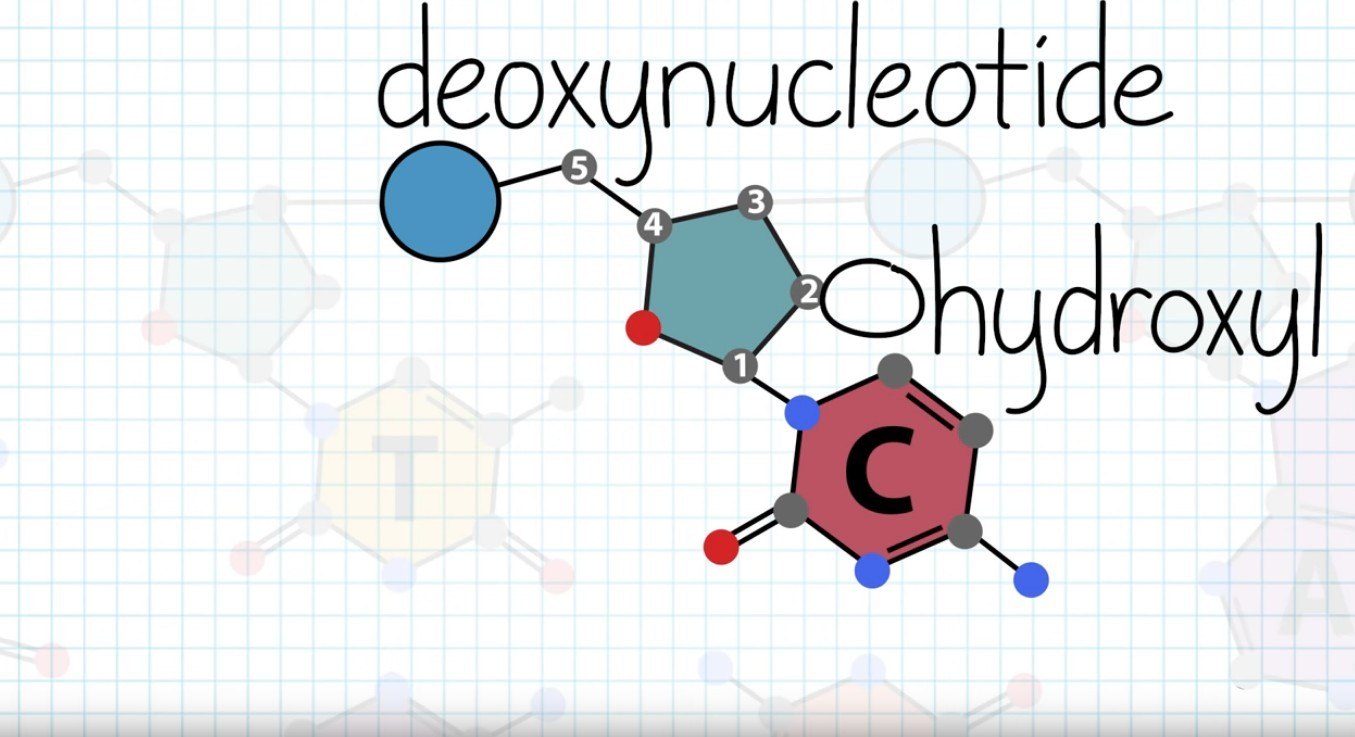
\includegraphics[width=\textwidth,height=0.7\textheight,keepaspectratio]{img/introduction/dna14.jpg}
		\label{img:mot2}
		\caption{Because of it, the nucleotides are also called deoxynucleotides.}
	\end{figure}
\end{frame}
%-------------------------------------------------------
%-------------------------------------------------------

%-------------------------------------------------------
%-------------------------------------------------------
\begin{frame}{DNA structure}{Overview}
	\begin{figure}[]
		\centering
		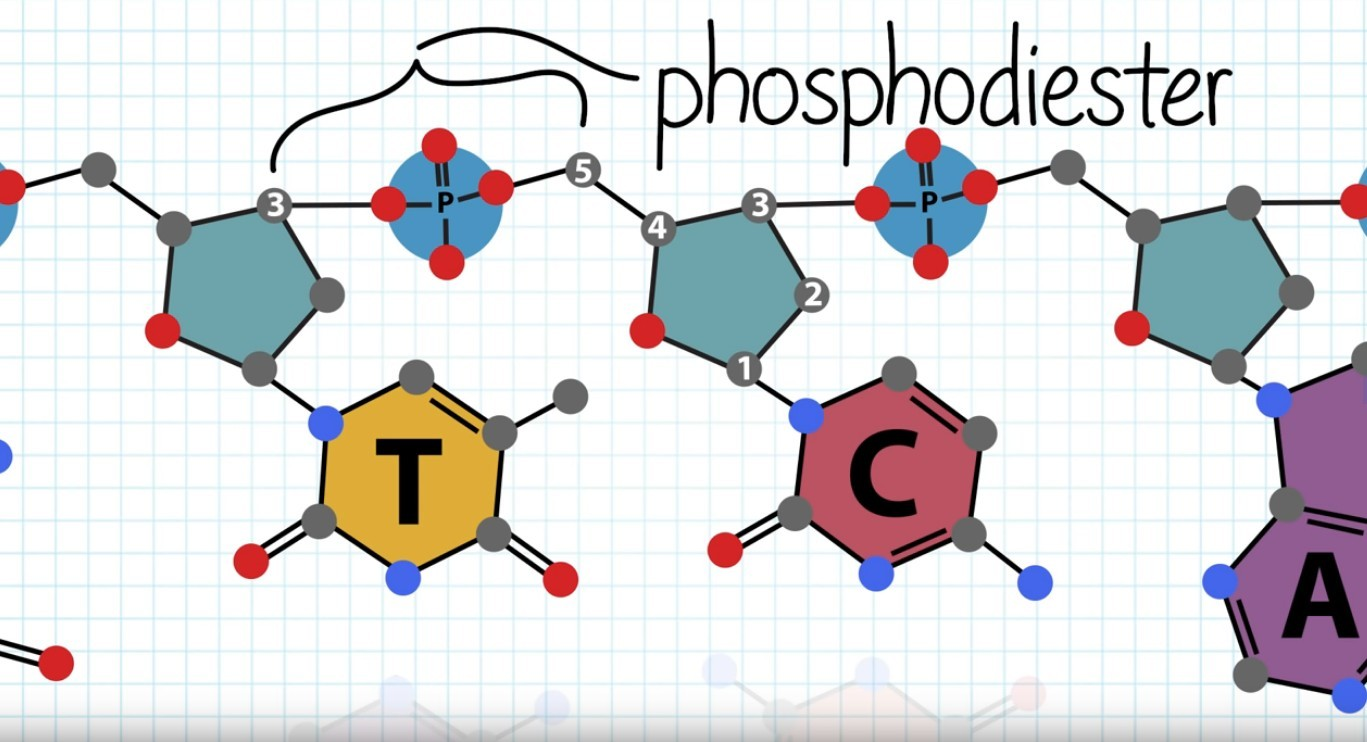
\includegraphics[width=\textwidth,height=0.7\textheight,keepaspectratio]{img/introduction/dna15.jpg}
		\label{img:mot2}
		\caption{The phosphate group of one nucleotide bind to the 3' oxygen of the neighbour nucleotide.}
	\end{figure}
\end{frame}
%-------------------------------------------------------
%-------------------------------------------------------

%-------------------------------------------------------
%-------------------------------------------------------
\begin{frame}{DNA structure}{Overview}
	\begin{figure}[]
		\centering
		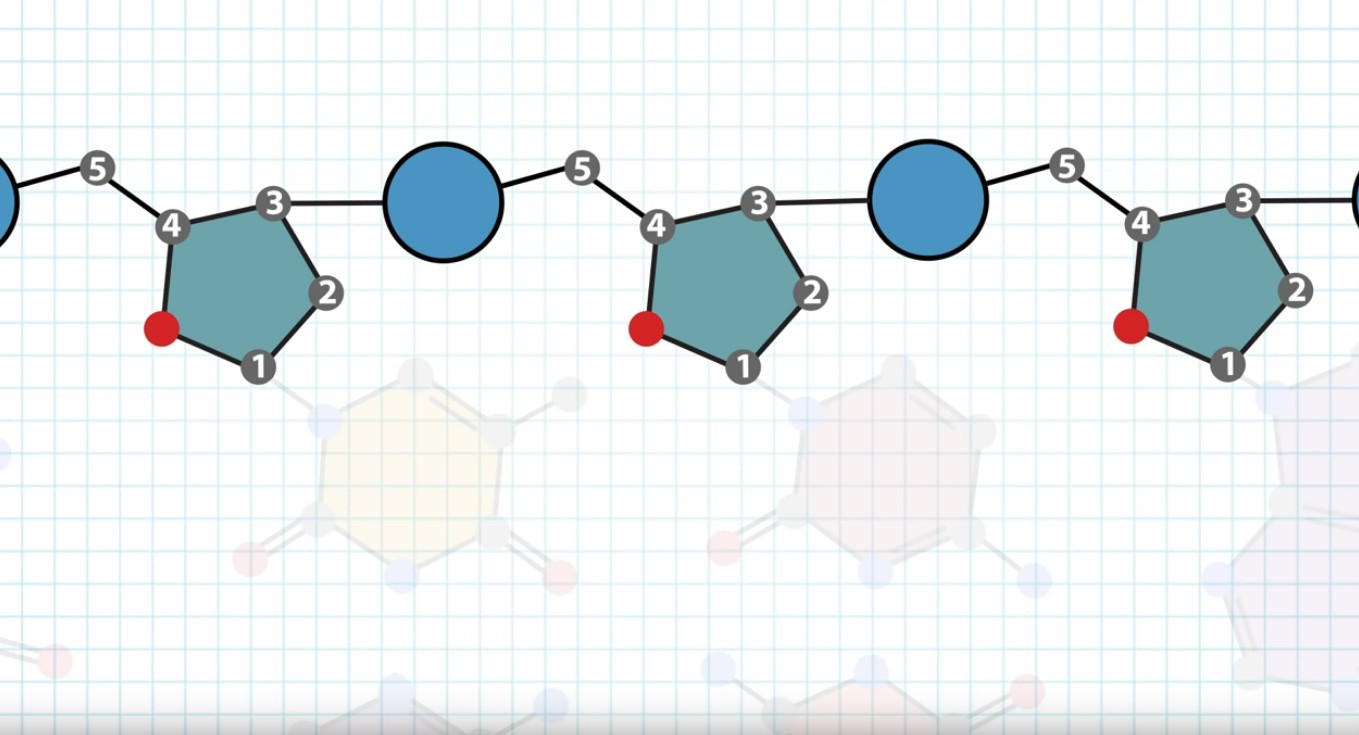
\includegraphics[width=\textwidth,height=0.7\textheight,keepaspectratio]{img/introduction/dna16.jpg}
		\label{img:mot2}
		\caption{The carbon number numbering is key to describe the directionality of the DNA strand, 5' to 3'.}
	\end{figure}
\end{frame}
%-------------------------------------------------------
%-------------------------------------------------------

%-------------------------------------------------------
%-------------------------------------------------------
\begin{frame}{DNA structure}{Overview}
	\begin{figure}[]
		\centering
		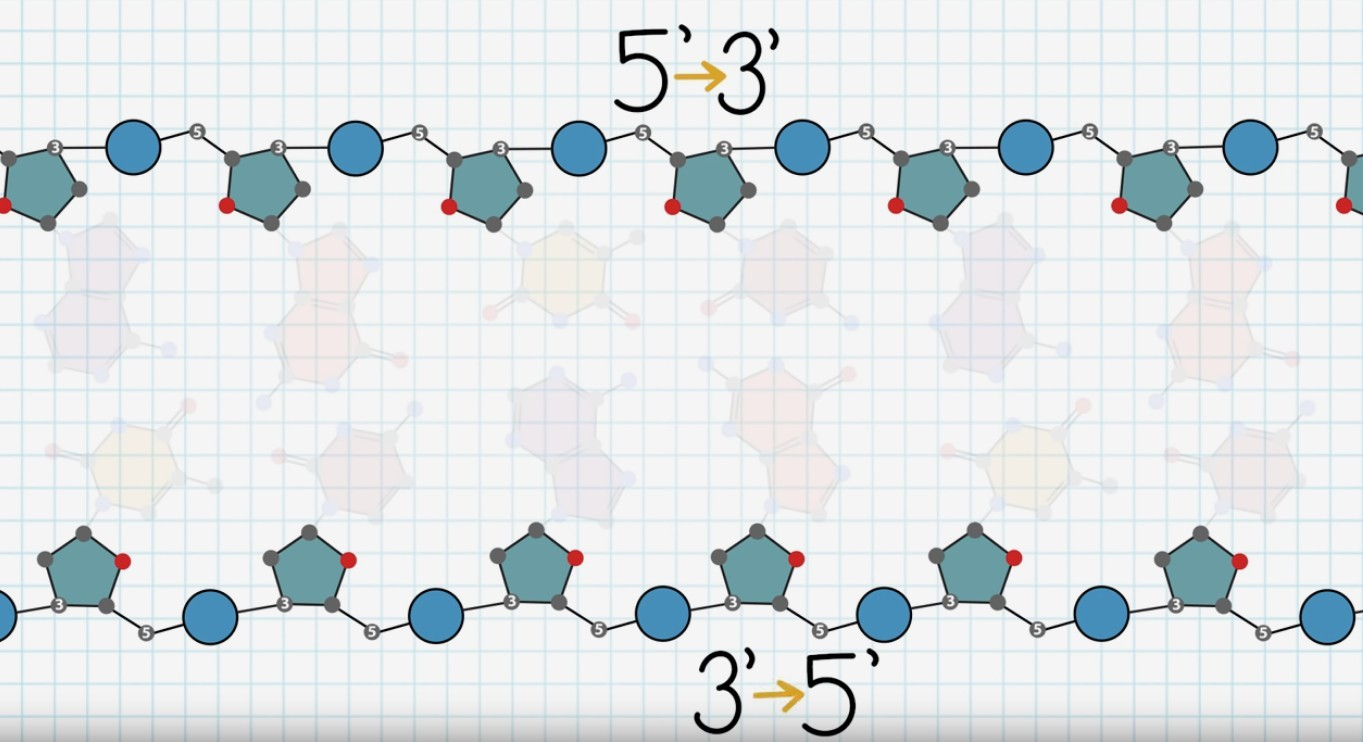
\includegraphics[width=\textwidth,height=0.7\textheight,keepaspectratio]{img/introduction/dna17.jpg}
		\label{img:mot2}
		\caption{The directionality od DNA, change in the top and bottom strand. It is also named Watson and Crick. }
	\end{figure}
\end{frame}
%-------------------------------------------------------
%-------------------------------------------------------

%-------------------------------------------------------
%-------------------------------------------------------
\begin{frame}{DNA structure}{Overview}
	\begin{figure}[]
		\centering
		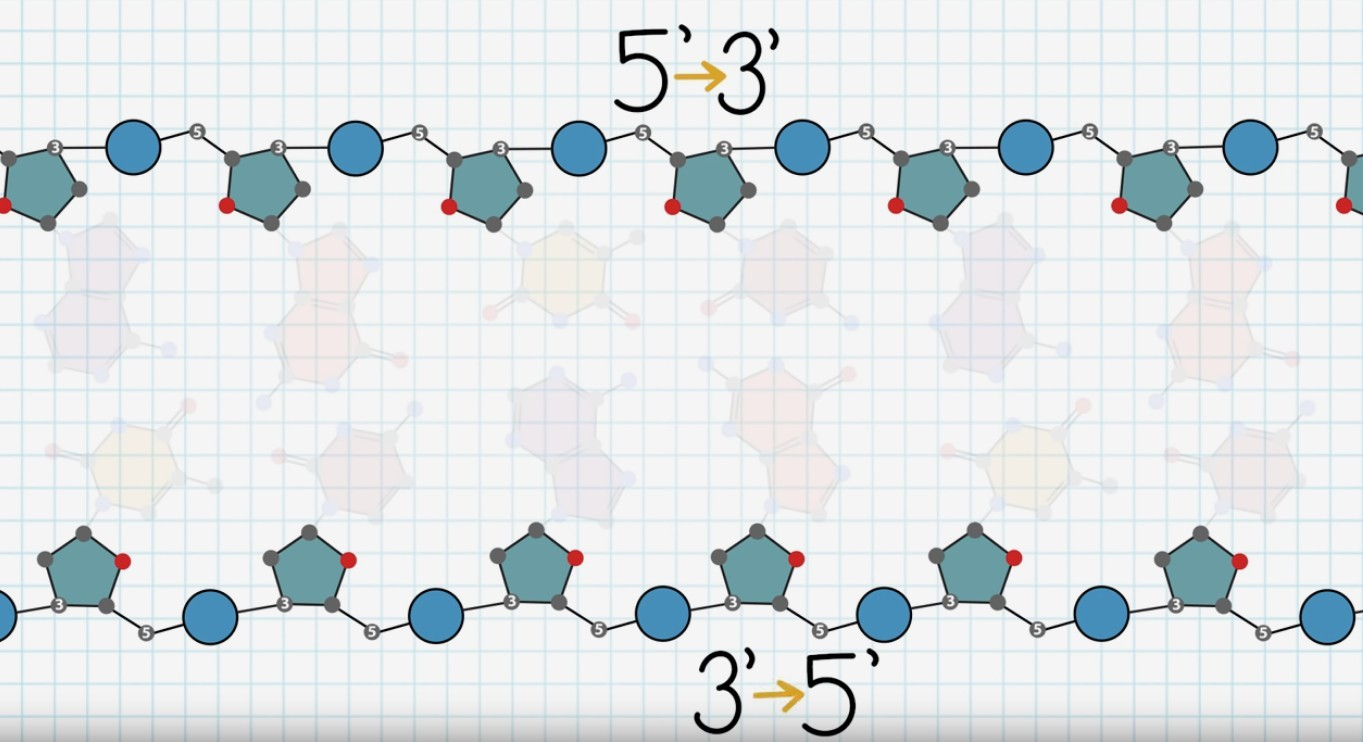
\includegraphics[width=\textwidth,height=0.7\textheight,keepaspectratio]{img/introduction/dna17.jpg}
		\label{img:mot2}
		\caption{The directionality od DNA, change in the top and bottom strand. It is also named Watson and Crick. }
	\end{figure}
\end{frame}
%-------------------------------------------------------
%-------------------------------------------------------

%-------------------------------------------------------
%-------------------------------------------------------
\begin{frame}{DNA structure}{Overview}
	\begin{figure}[]
		\centering
		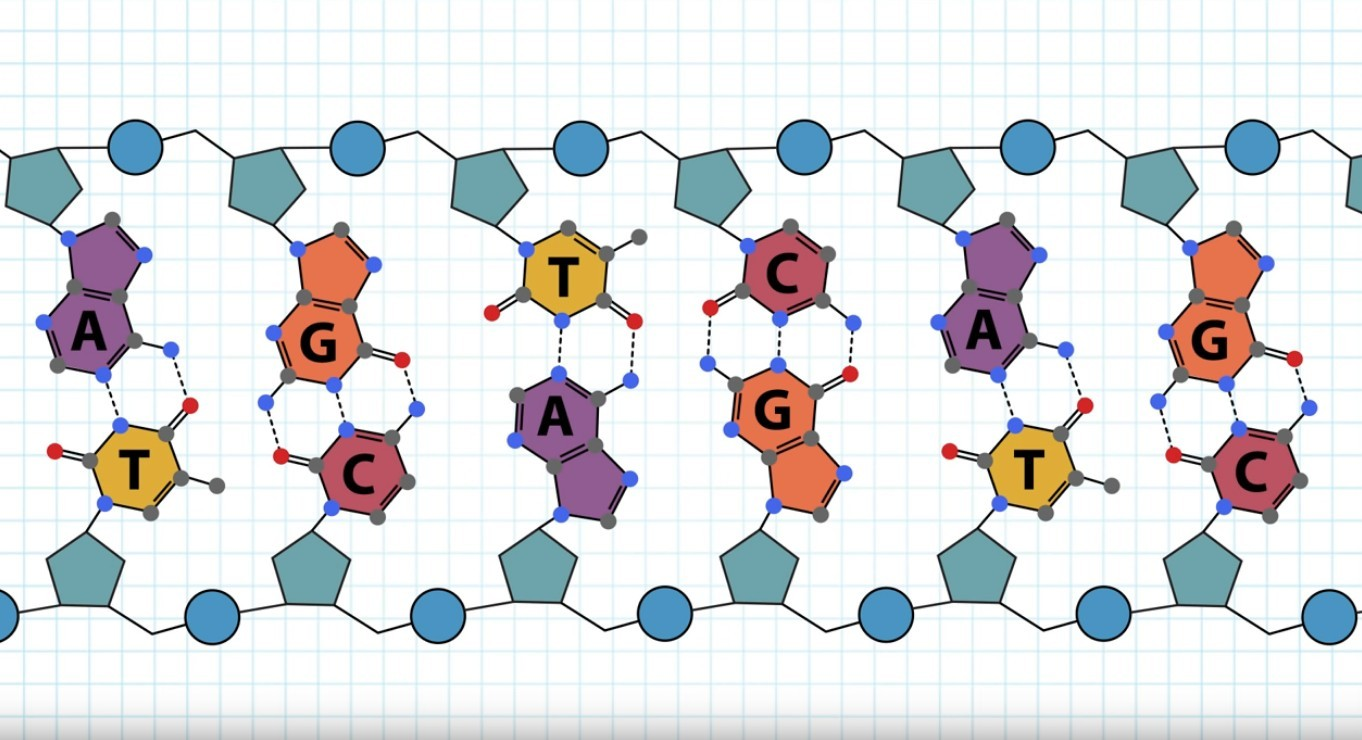
\includegraphics[width=\textwidth,height=0.7\textheight,keepaspectratio]{img/introduction/dna18.jpg}
		\label{img:mot2}
		\caption{The two strand interact through non-covalent hydrogen between the bases.}
	\end{figure}
\end{frame}
%-------------------------------------------------------
%-------------------------------------------------------

%-------------------------------------------------------
%-------------------------------------------------------
\begin{frame}{DNA structure}{Overview}
	\begin{figure}[]
		\centering
		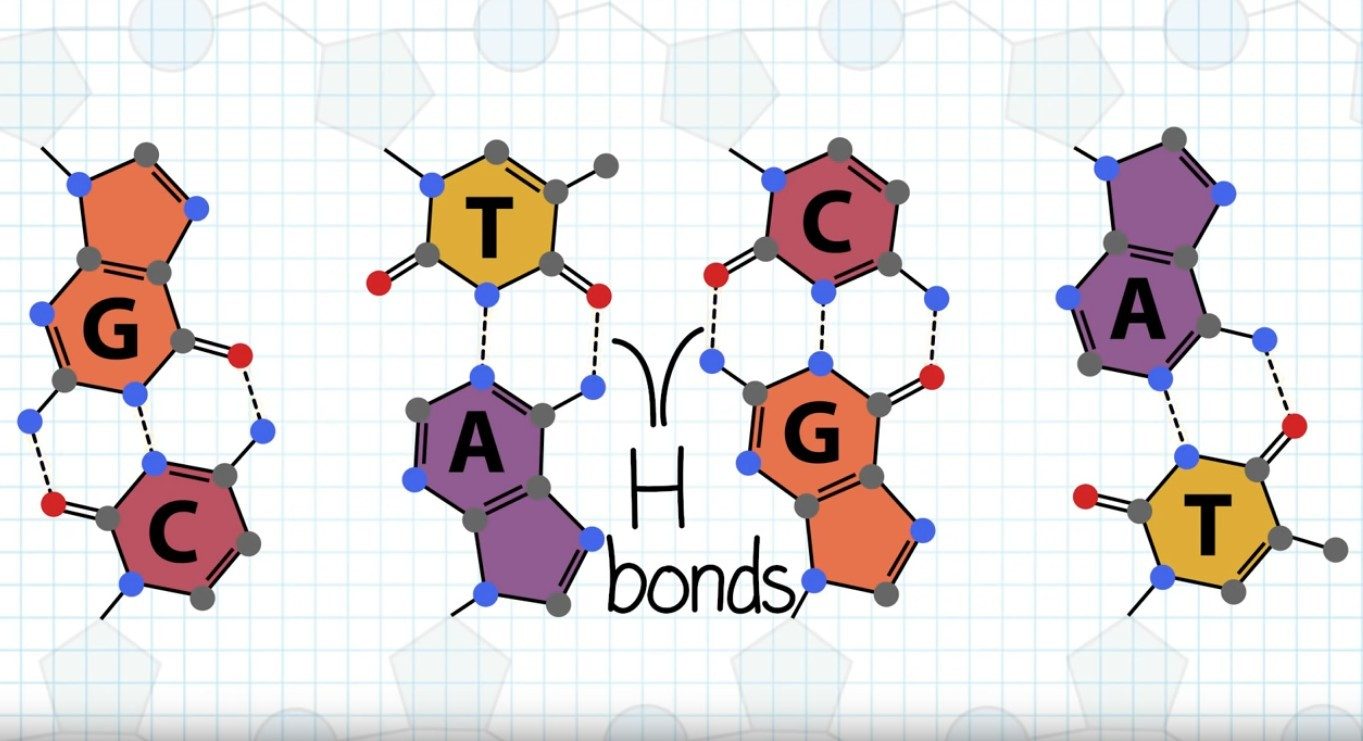
\includegraphics[width=\textwidth,height=0.7\textheight,keepaspectratio]{img/introduction/dna19.jpg}
		\label{img:mot2}
		\caption{Each base forms multiple hydrogen bonds with its complementary base on the opposite strand.}
	\end{figure}
\end{frame}
%-------------------------------------------------------
%-------------------------------------------------------

%-------------------------------------------------------
%-------------------------------------------------------
\begin{frame}{DNA structure}{Overview}
	\begin{figure}[]
		\centering
		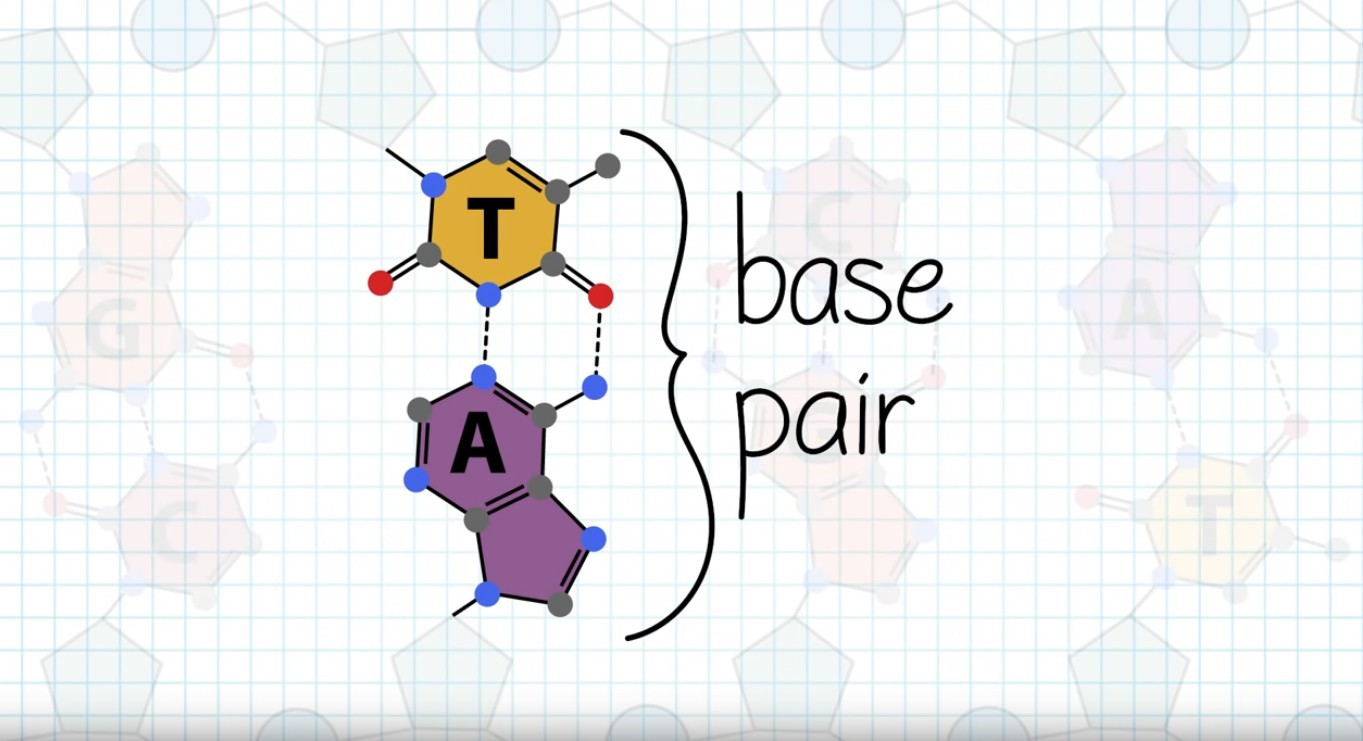
\includegraphics[width=\textwidth,height=0.7\textheight,keepaspectratio]{img/introduction/dna20.jpg}
		\label{img:mot2}
		\caption{Each unit is called a base pair.}
	\end{figure}
\end{frame}
%-------------------------------------------------------
%-------------------------------------------------------

%-------------------------------------------------------
%-------------------------------------------------------
\begin{frame}{DNA structure}{Overview}
	\begin{figure}[]
		\centering
		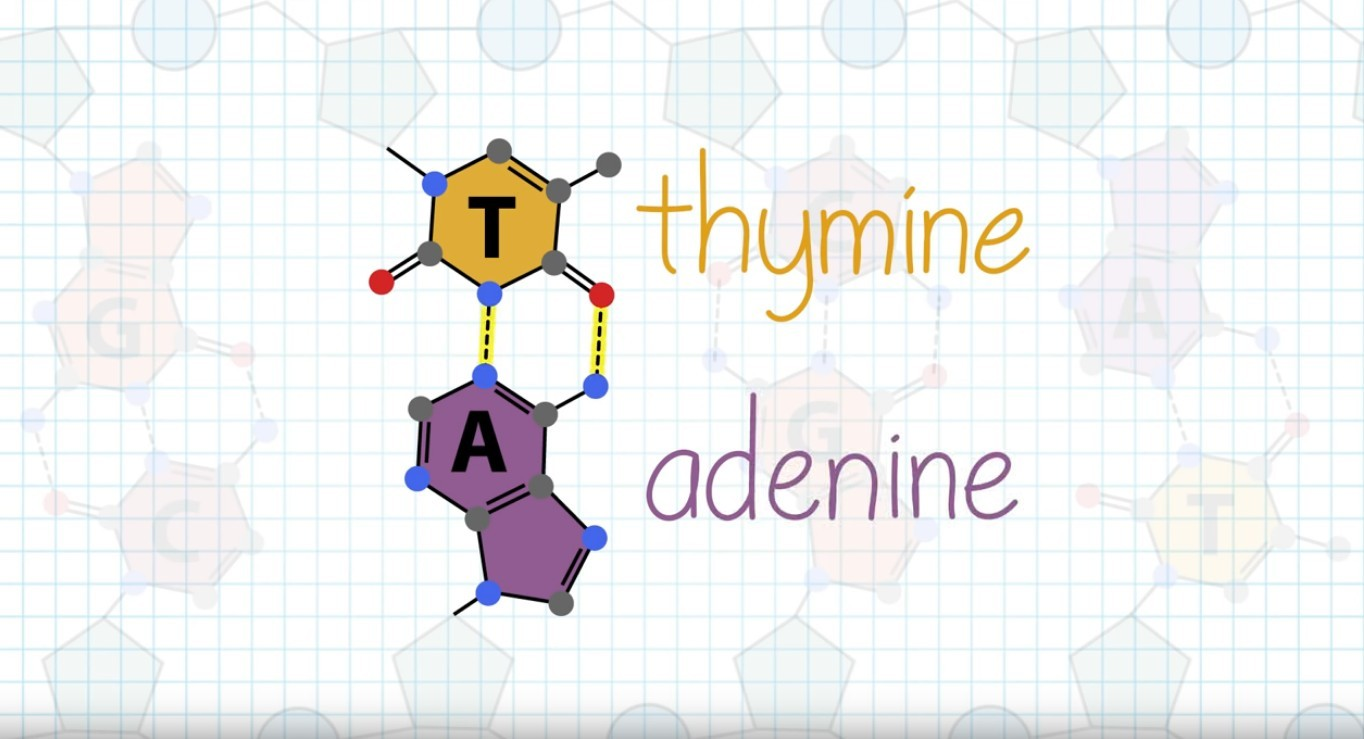
\includegraphics[width=\textwidth,height=0.7\textheight,keepaspectratio]{img/introduction/dna21.jpg}
		\label{img:mot2}
		\caption{Thymine preferentially pairs with Adenine with two hydrogen bonds.}
	\end{figure}
\end{frame}
%-------------------------------------------------------
%-------------------------------------------------------

%-------------------------------------------------------
%-------------------------------------------------------
\begin{frame}{DNA structure}{Overview}
	\begin{figure}[]
		\centering
		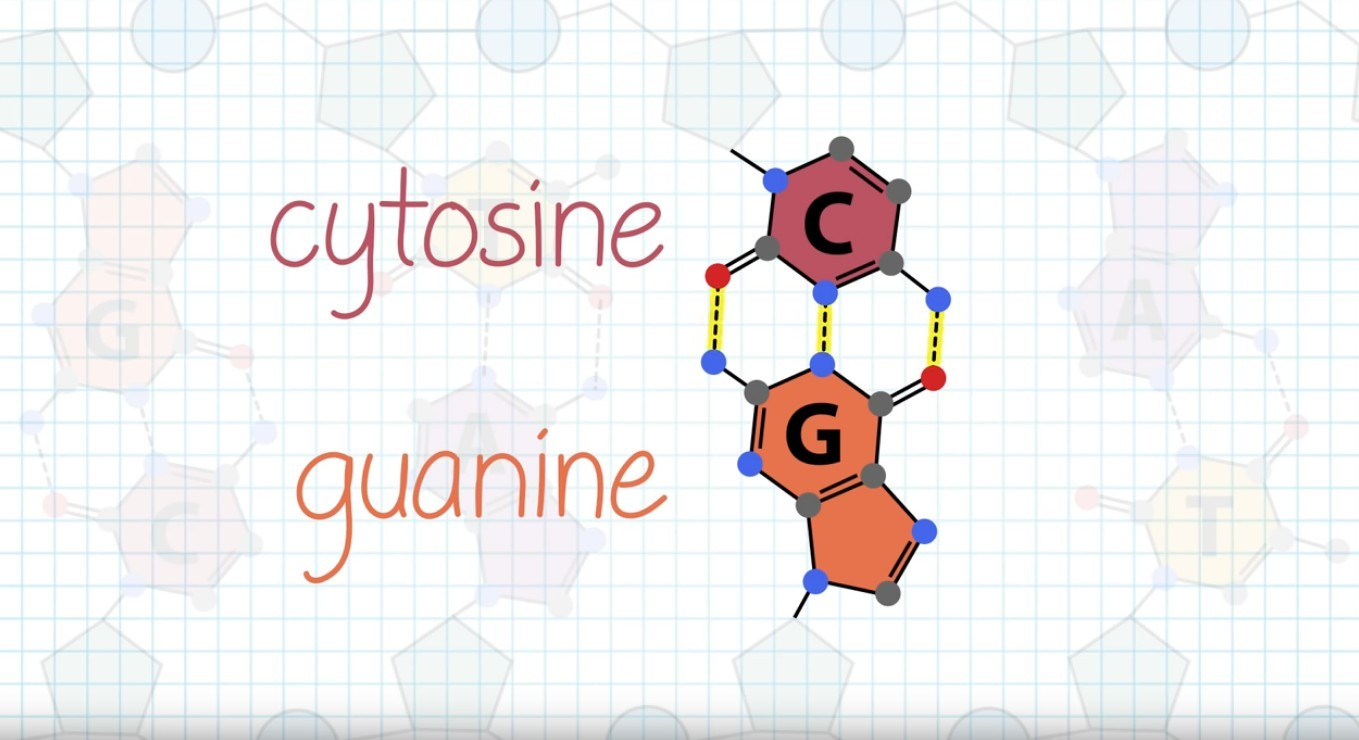
\includegraphics[width=\textwidth,height=0.7\textheight,keepaspectratio]{img/introduction/dna22.jpg}
		\label{img:mot2}
		\caption{Cytosine preferentially pairs with Guanine with three hydrogen bonds.}
	\end{figure}
\end{frame}
%-------------------------------------------------------
%-------------------------------------------------------

%-------------------------------------------------------
%-------------------------------------------------------
\begin{frame}{DNA structure}{Overview}
	\begin{figure}[]
		\centering
		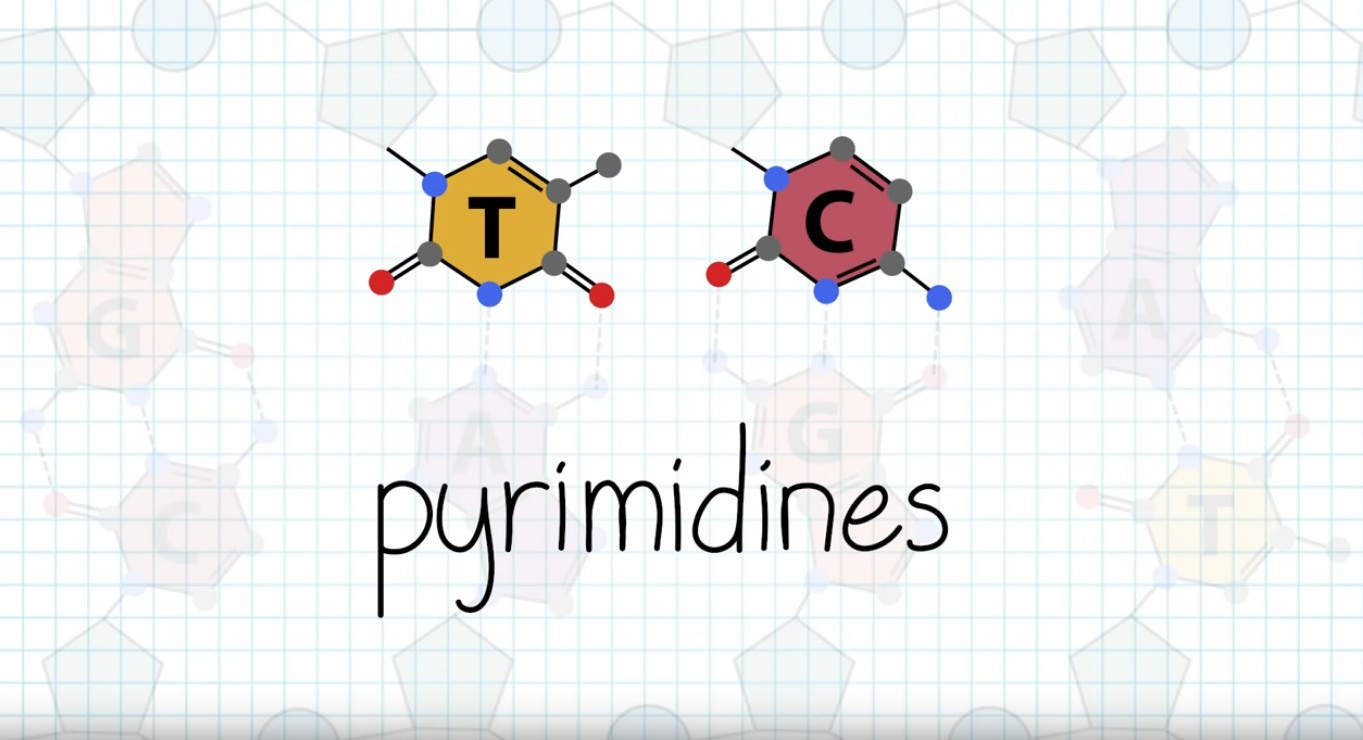
\includegraphics[width=\textwidth,height=0.7\textheight,keepaspectratio]{img/introduction/dna23.jpg}
		\label{img:mot2}
		\caption{Thymine and Cytosine are called pyrimidines characterized by a single ring structure.}
	\end{figure}
\end{frame}
%-------------------------------------------------------
%-------------------------------------------------------

%-------------------------------------------------------
%-------------------------------------------------------
\begin{frame}{DNA structure}{Overview}
	\begin{figure}[]
		\centering
		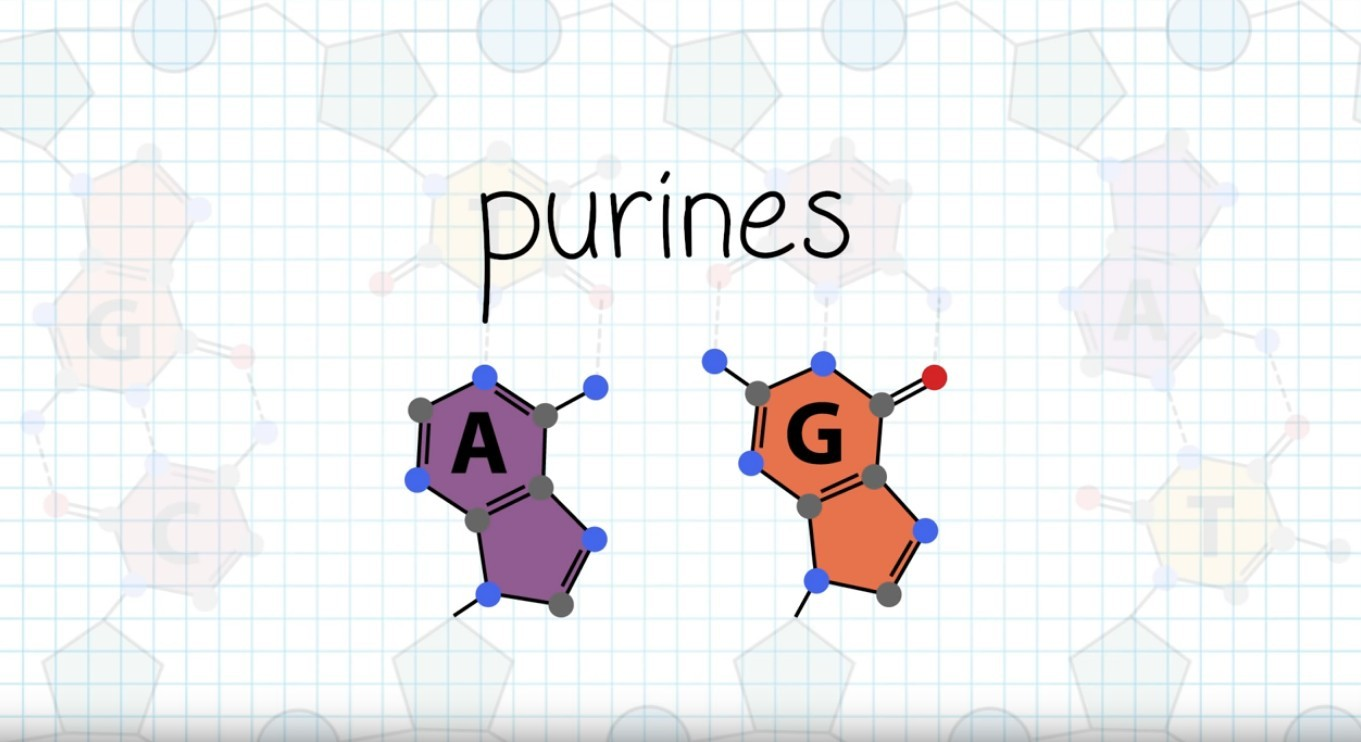
\includegraphics[width=\textwidth,height=0.7\textheight,keepaspectratio]{img/introduction/dna24.jpg}
		\label{img:mot2}
		\caption{Adenine and Guanine are called purines which have double rings.}
	\end{figure}
\end{frame}
%-------------------------------------------------------
%-------------------------------------------------------


%%%%%%%%%%%%%%%%%%%%%%%%%%%%%%%%%%%%%%%%%%%%%%%%%%%%%%%%%%%%%%%%%%%%%%%%%%%%%%%%%%%%%%%%%%%%%%%%%%%%%%%%%%%%%%%%
%%%%%%%%%%%%%%%%%%%%%%%%%%%%%%%%%%%%%%%%%%%%%%%%%%%%%%%%%%%%%%%%%%%%%%%%%%%%%%%%%%%%%%%%%%%%%%%%%%%%%%%%%%%%%%%%
%%%%%%%%%%%%%%%%%%%%%%%%%%%%%%%%%%%%%%%%%%%%%%%%%%%%%%%%%%%%%%%%%%%%%%%%%%%%%%%%%%%%%%%%%%%%%%%%%%%%%%%%%%%%%%%%
\subsection{DNA replication}
%%%%%%%%%%%%%%%%%%%%%%%%%%%%%%%%%%%%%%%%%%%%%%%%%%%%%%%%%%%%%%%%%%%%%%%%%%%%%%%%%%%%%%%%%%%%%%%%%%%%%%%%%%%%%%%%
%%%%%%%%%%%%%%%%%%%%%%%%%%%%%%%%%%%%%%%%%%%%%%%%%%%%%%%%%%%%%%%%%%%%%%%%%%%%%%%%%%%%%%%%%%%%%%%%%%%%%%%%%%%%%%%%
%%%%%%%%%%%%%%%%%%%%%%%%%%%%%%%%%%%%%%%%%%%%%%%%%%%%%%%%%%%%%%%%%%%%%%%%%%%%%%%%%%%%%%%%%%%%%%%%%%%%%%%%%%%%%%%%

%-------------------------------------------------------
%-------------------------------------------------------
\begin{frame}{DNA replication}{Overview}
\begin{block}{}
	DNA replication is the biological process of producing two identical replicas of DNA from one original DNA molecule.
\end{block}

\begin{block}{}
	The following content is extracted from the video \href{https://www.youtube.com/watch?v=TNKWgcFPHqw}{\textbf{DNA replication - 3D}} \cite{MITx2020}.
\end{block}
\end{frame}
%-------------------------------------------------------
%-------------------------------------------------------

%-------------------------------------------------------
%-------------------------------------------------------
\begin{frame}{DNA replication}{Overview}
	\begin{figure}[]
		\centering
		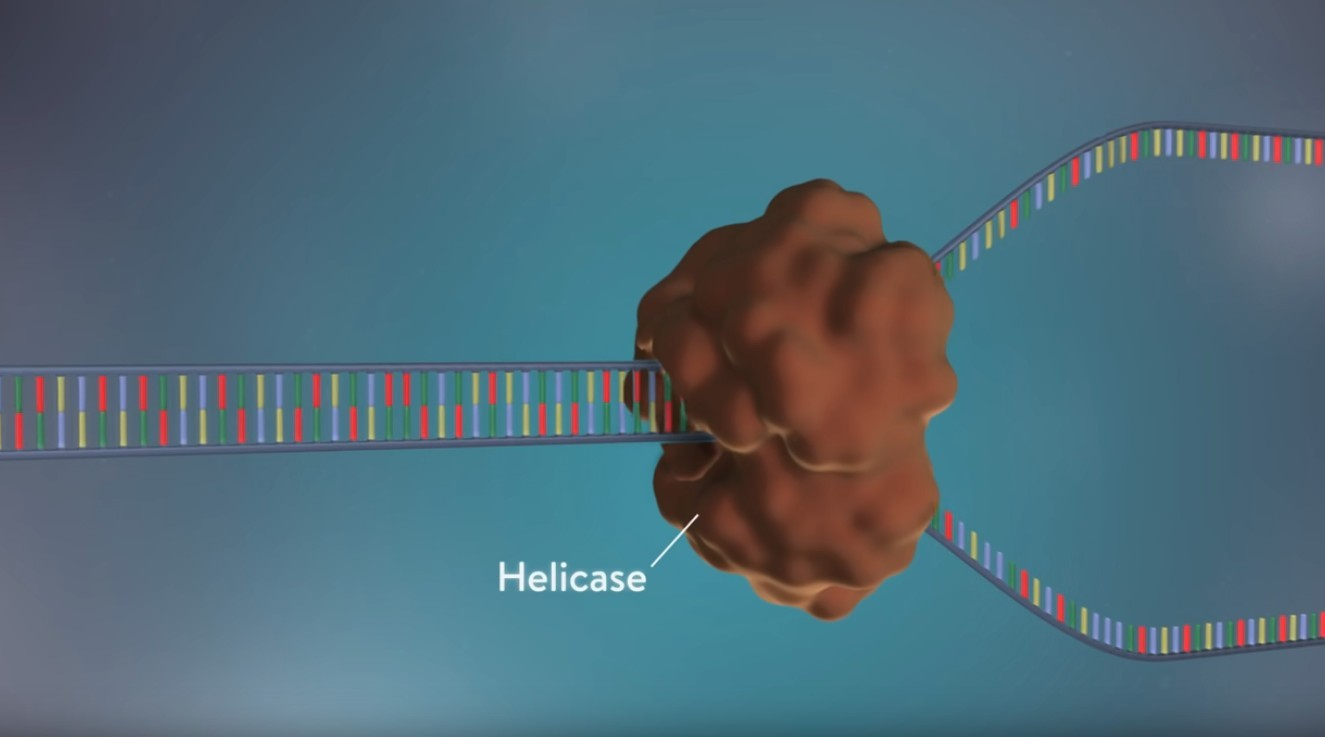
\includegraphics[width=\textwidth,height=0.6\textheight,keepaspectratio]{img/introduction/dna30.jpg}
		\label{img:mot2}
		\caption{The first step in DNA replication is to unzip the double helix by an enzyme called \textbf{helicase}.}
	\end{figure}
\end{frame}
%-------------------------------------------------------
%-------------------------------------------------------

%-------------------------------------------------------
%-------------------------------------------------------
\begin{frame}{DNA replication}{Overview}
	\begin{figure}[]
		\centering
		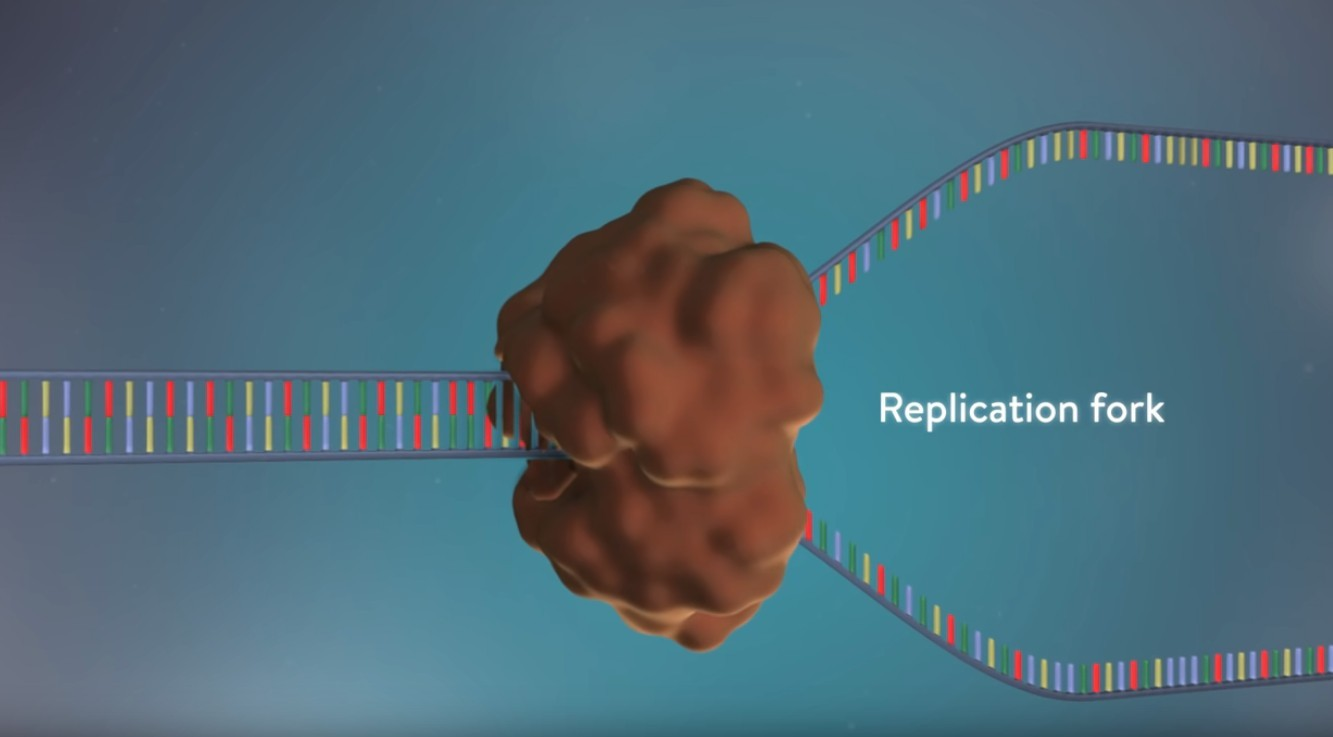
\includegraphics[width=\textwidth,height=0.6\textheight,keepaspectratio]{img/introduction/dna31.jpg}
		\label{img:mot2}
		\caption{The separation of the two single strands of DNA creates a \textbf{Y} shape called a replication \textbf{fork}.}
	\end{figure}
\end{frame}
%-------------------------------------------------------
%-------------------------------------------------------

%-------------------------------------------------------
%-------------------------------------------------------
\begin{frame}{DNA replication}{Overview}
	\begin{figure}[]
		\centering
		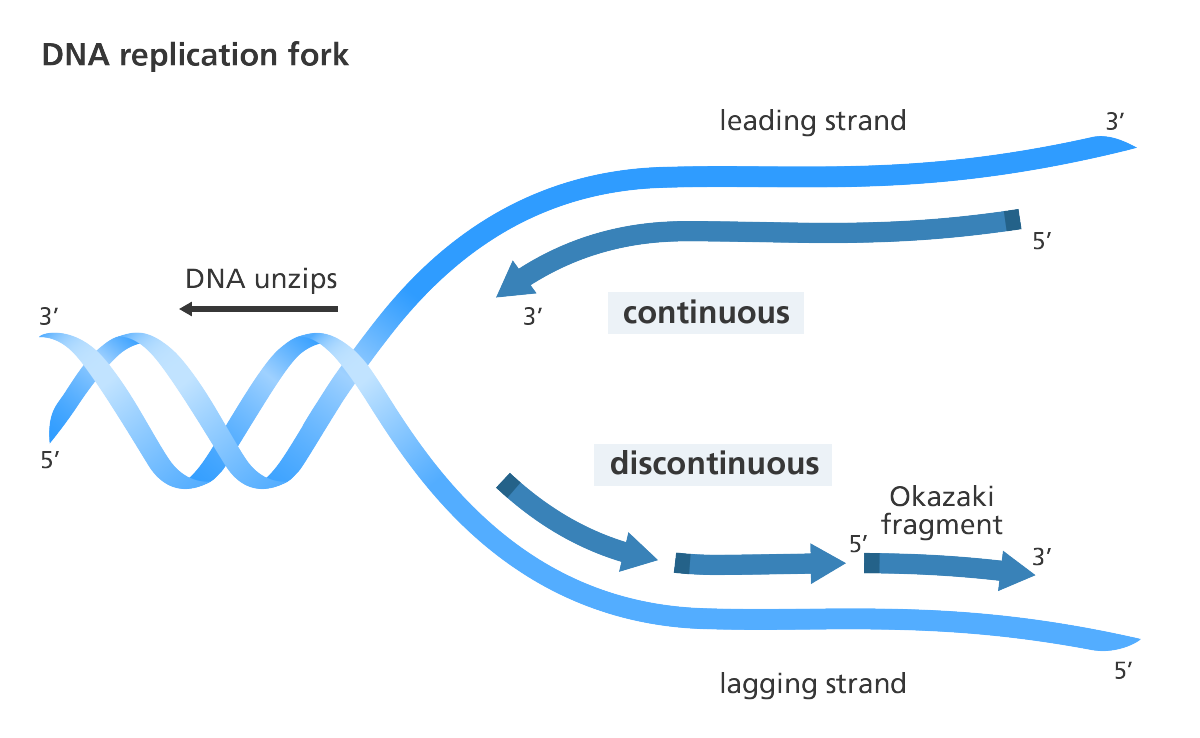
\includegraphics[width=\textwidth,height=0.6\textheight,keepaspectratio]{img/introduction/dna32.png}
		\label{img:mot2}
		\caption{One of the strands is oriented in the 3’ to 5’ direction (leading strand). The other strand is oriented in the 5’ to 3’ direction (lagging strand).}
	\end{figure}
\end{frame}
%-------------------------------------------------------
%-------------------------------------------------------

%-------------------------------------------------------
%-------------------------------------------------------
\begin{frame}{DNA replication}{Overview}
	\begin{figure}[]
		\centering
		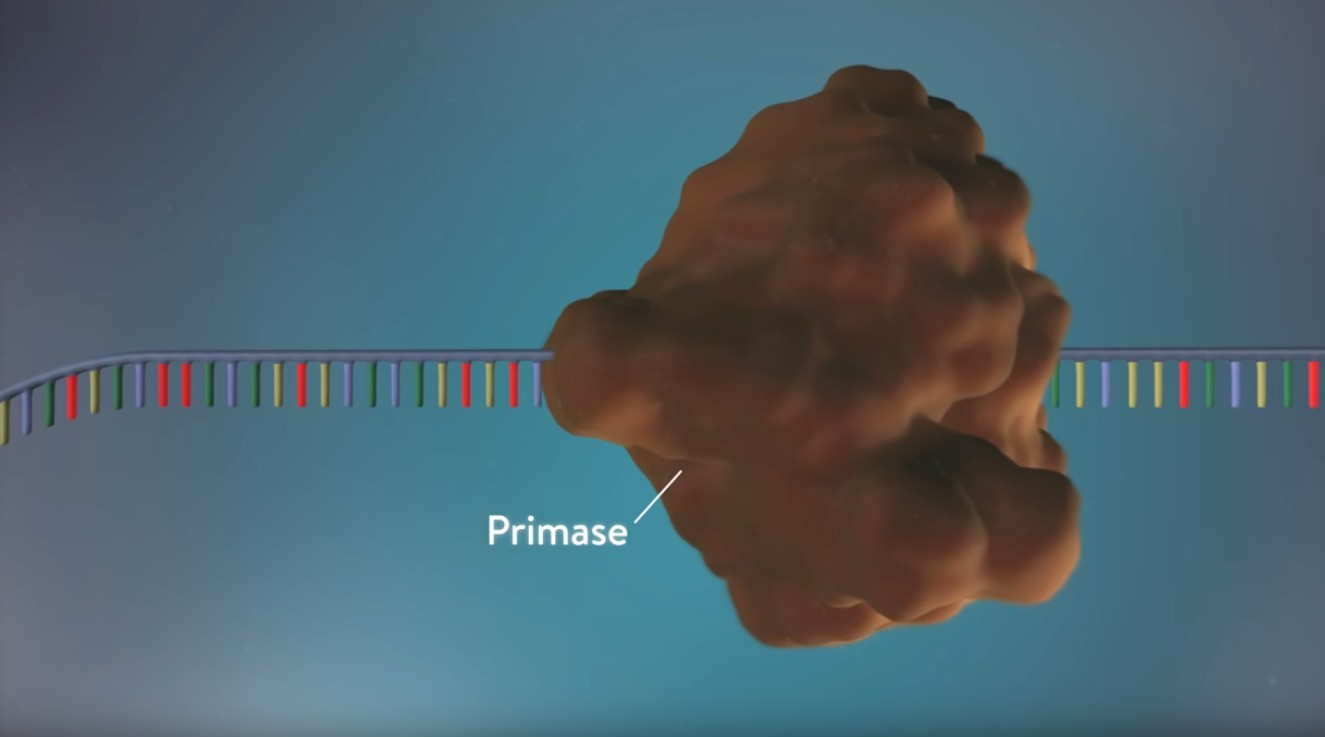
\includegraphics[width=\textwidth,height=0.6\textheight,keepaspectratio]{img/introduction/dna33.jpg}
		\label{img:mot2}
		\caption{In the leading strand, an enzyme called \textbf{primase} start the process.}
	\end{figure}
\end{frame}
%-------------------------------------------------------
%-------------------------------------------------------


%-------------------------------------------------------
%-------------------------------------------------------
\begin{frame}{DNA replication}{Overview}
	\begin{figure}[]
		\centering
		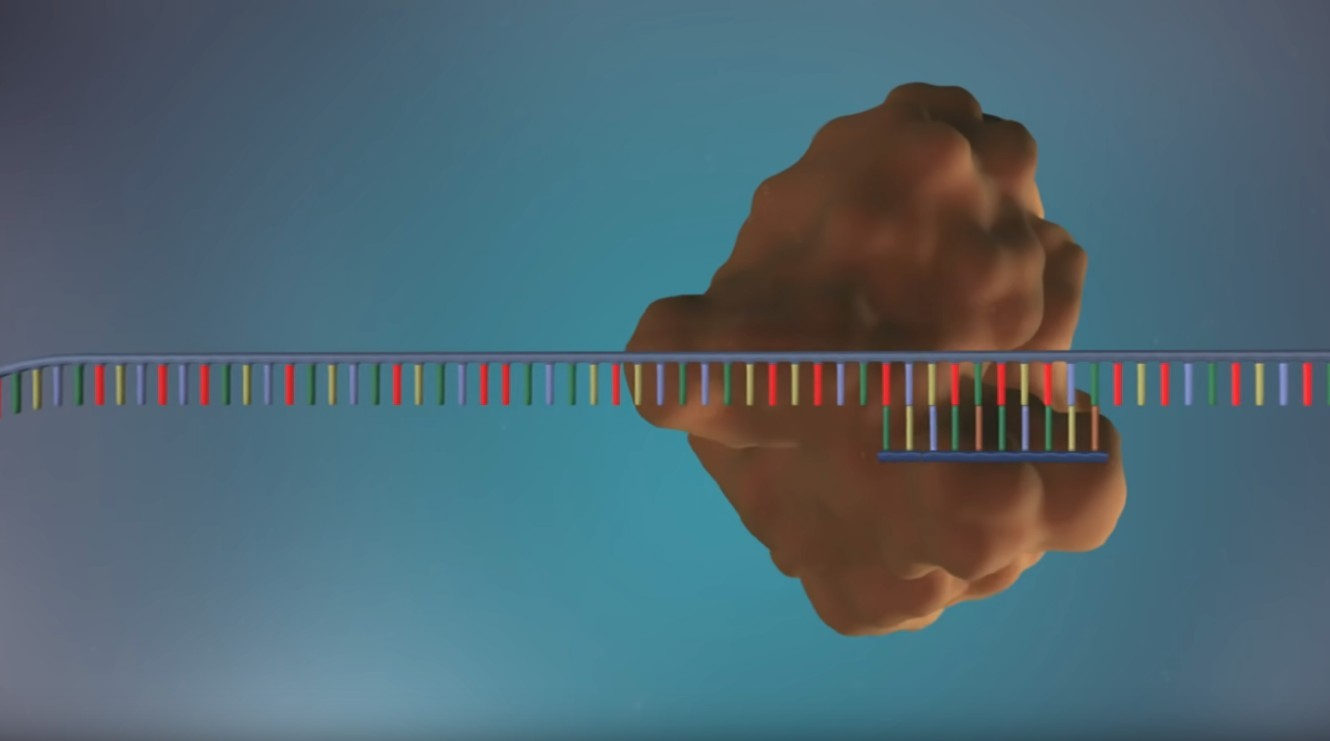
\includegraphics[width=\textwidth,height=0.6\textheight,keepaspectratio]{img/introduction/dna34.jpg}
		\label{img:mot2}
		\caption{This enzyme makes a small piece of RNA.}
	\end{figure}
\end{frame}
%-------------------------------------------------------
%-------------------------------------------------------

%-------------------------------------------------------
%-------------------------------------------------------
\begin{frame}{DNA replication}{Overview}
	\begin{figure}[]
		\centering
		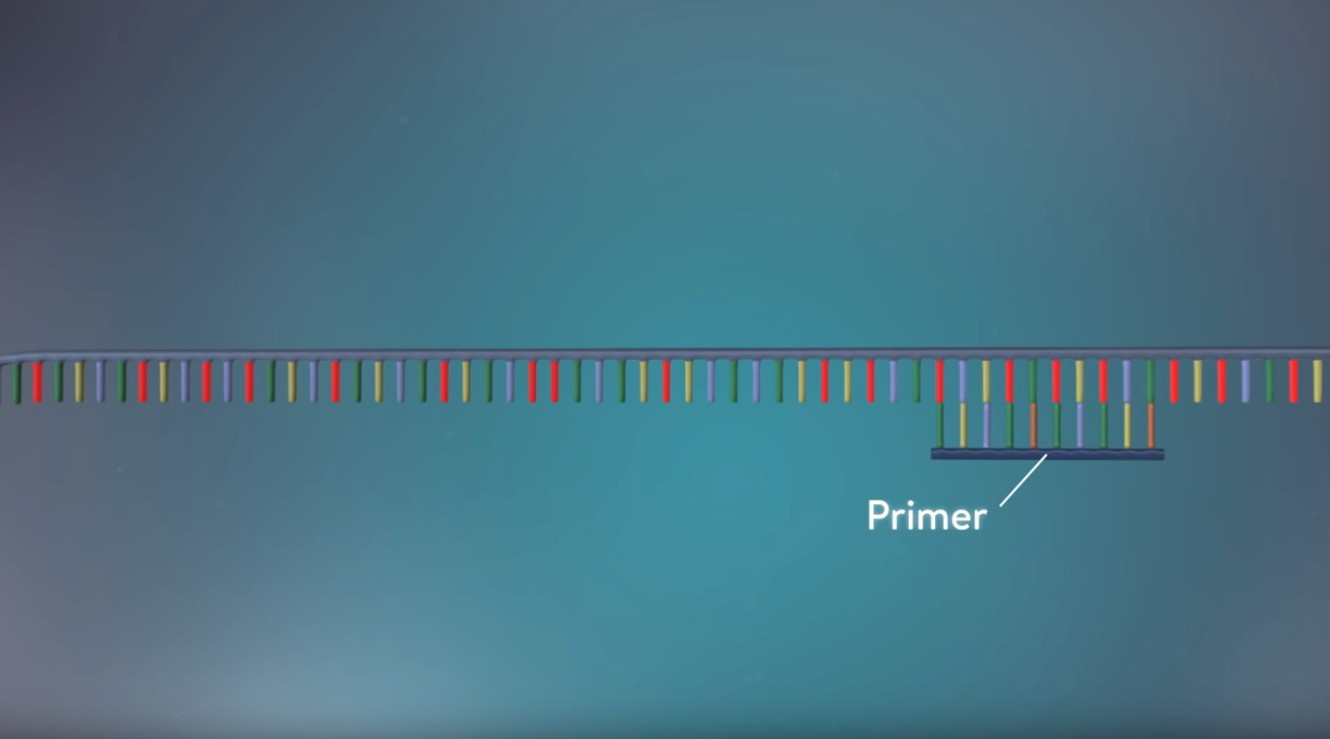
\includegraphics[width=\textwidth,height=0.6\textheight,keepaspectratio]{img/introduction/dna35.jpg}
		\label{img:mot2}
		\caption{This small piece of RNA is called \textbf{Primer}. This marks the starting point for the construction of the new strand of DNA}
	\end{figure}
\end{frame}
%-------------------------------------------------------
%-------------------------------------------------------

%-------------------------------------------------------
%-------------------------------------------------------
\begin{frame}{DNA replication}{Overview}
	\begin{figure}[]
		\centering
		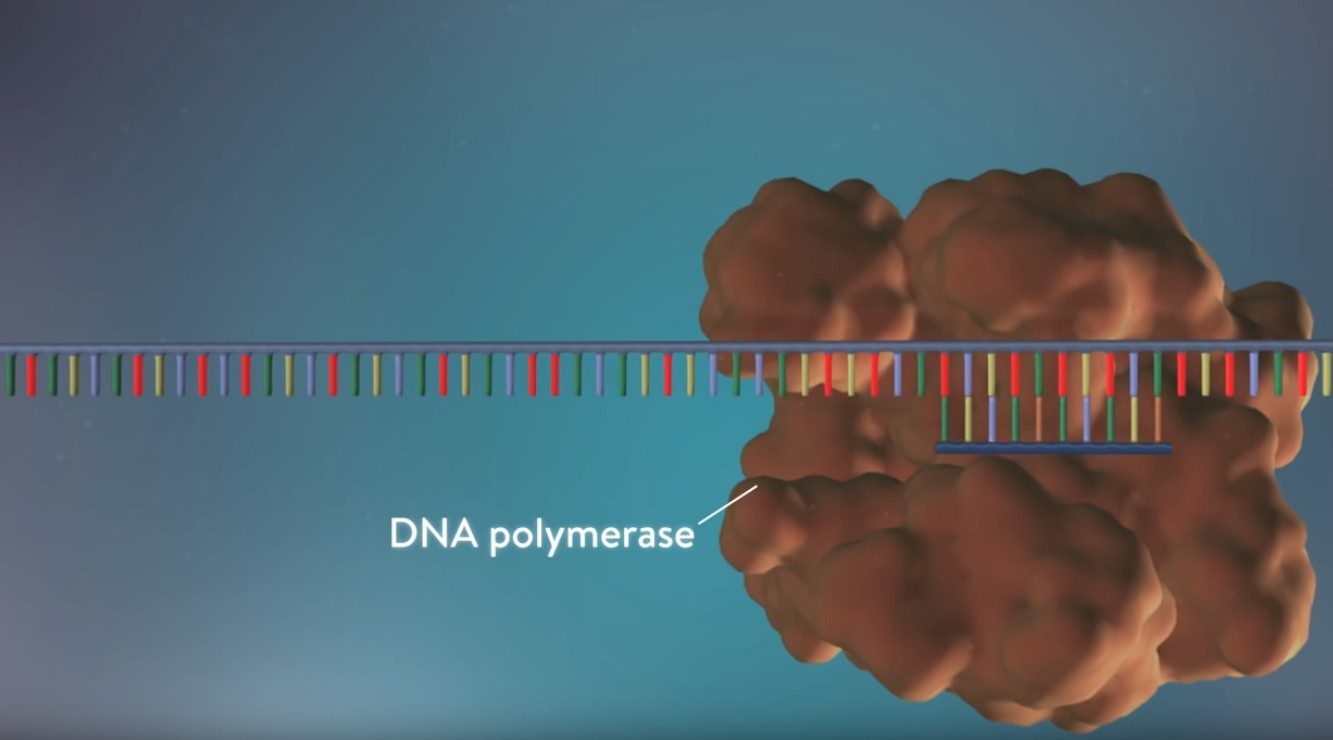
\includegraphics[width=\textwidth,height=0.6\textheight,keepaspectratio]{img/introduction/dna36.jpg}
		\label{img:mot2}
		\caption{An enzyme called \textbf{DNA polymerase} binds to the primer and will make the new strand of DNA.}
	\end{figure}
\end{frame}
%-------------------------------------------------------
%-------------------------------------------------------



%-------------------------------------------------------
%-------------------------------------------------------
\begin{frame}{DNA replication}{Overview}
	\begin{figure}[]
		\centering
		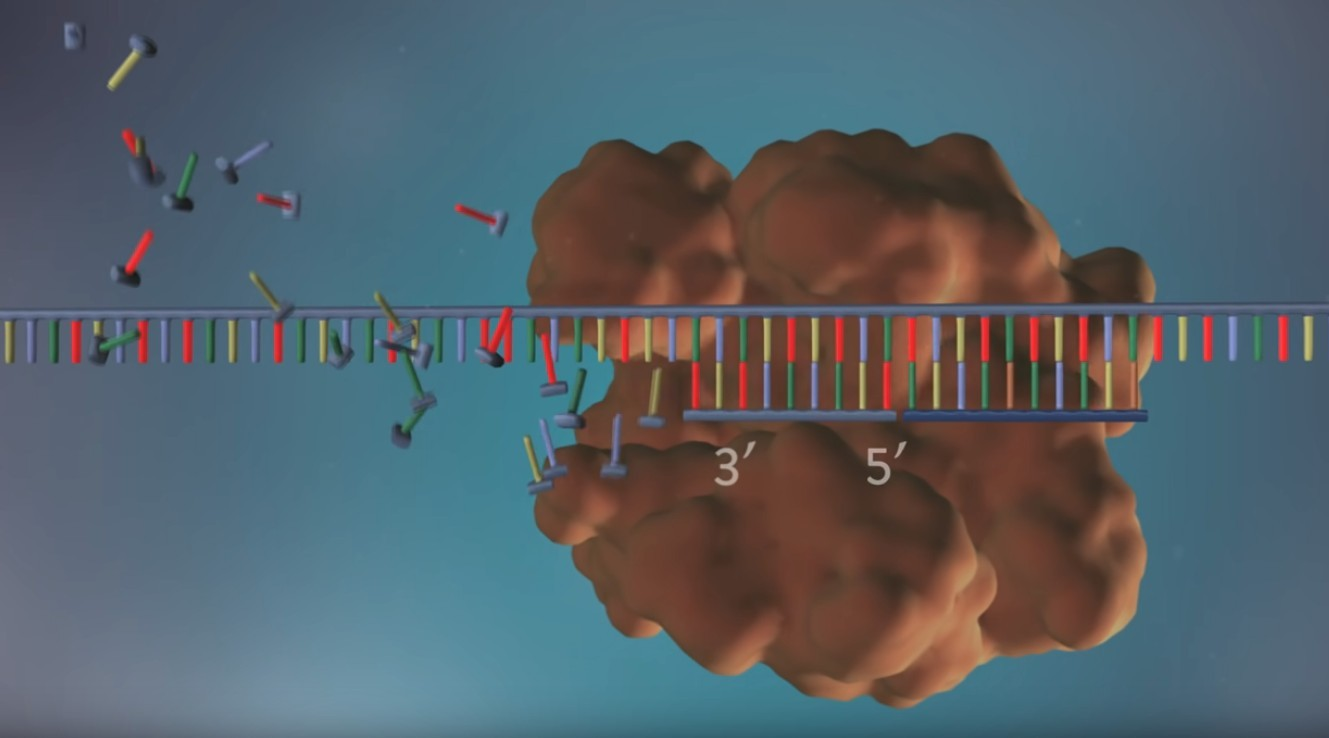
\includegraphics[width=\textwidth,height=0.6\textheight,keepaspectratio]{img/introduction/dna37.jpg}
		\label{img:mot2}
		\caption{DNA polymerase add DNA bases in 5' to 3' direction. The \textbf{leading strand} is made continuously.}
	\end{figure}
\end{frame}
%-------------------------------------------------------
%-------------------------------------------------------


%-------------------------------------------------------
%-------------------------------------------------------
\begin{frame}{DNA replication}{Overview}
	\begin{figure}[]
		\centering
		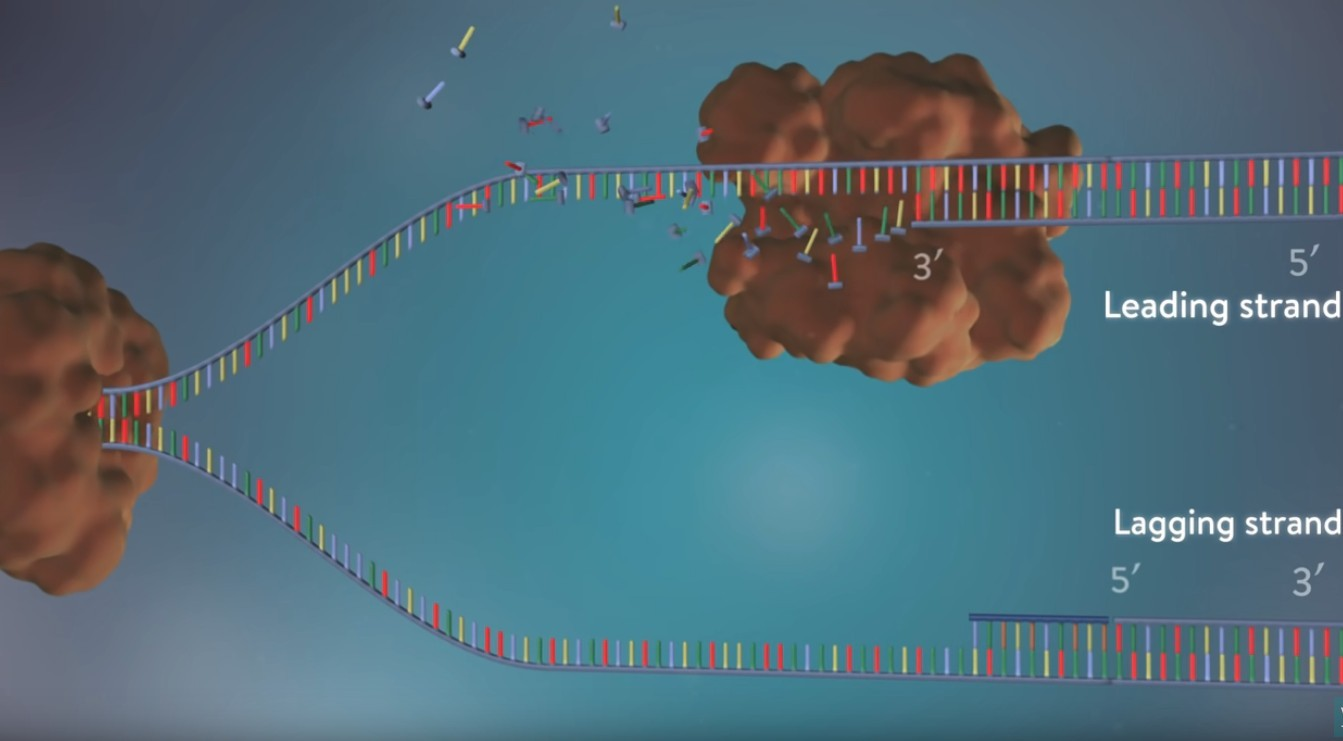
\includegraphics[width=\textwidth,height=0.6\textheight,keepaspectratio]{img/introduction/dna38.jpg}
		\label{img:mot2}
		\caption{The leading strand is made continuously but the lagging strand can not because it runs in the opposite direction.}
	\end{figure}
\end{frame}
%-------------------------------------------------------
%-------------------------------------------------------


%-------------------------------------------------------
%-------------------------------------------------------
\begin{frame}{DNA replication}{Overview}
	\begin{figure}[]
		\centering
		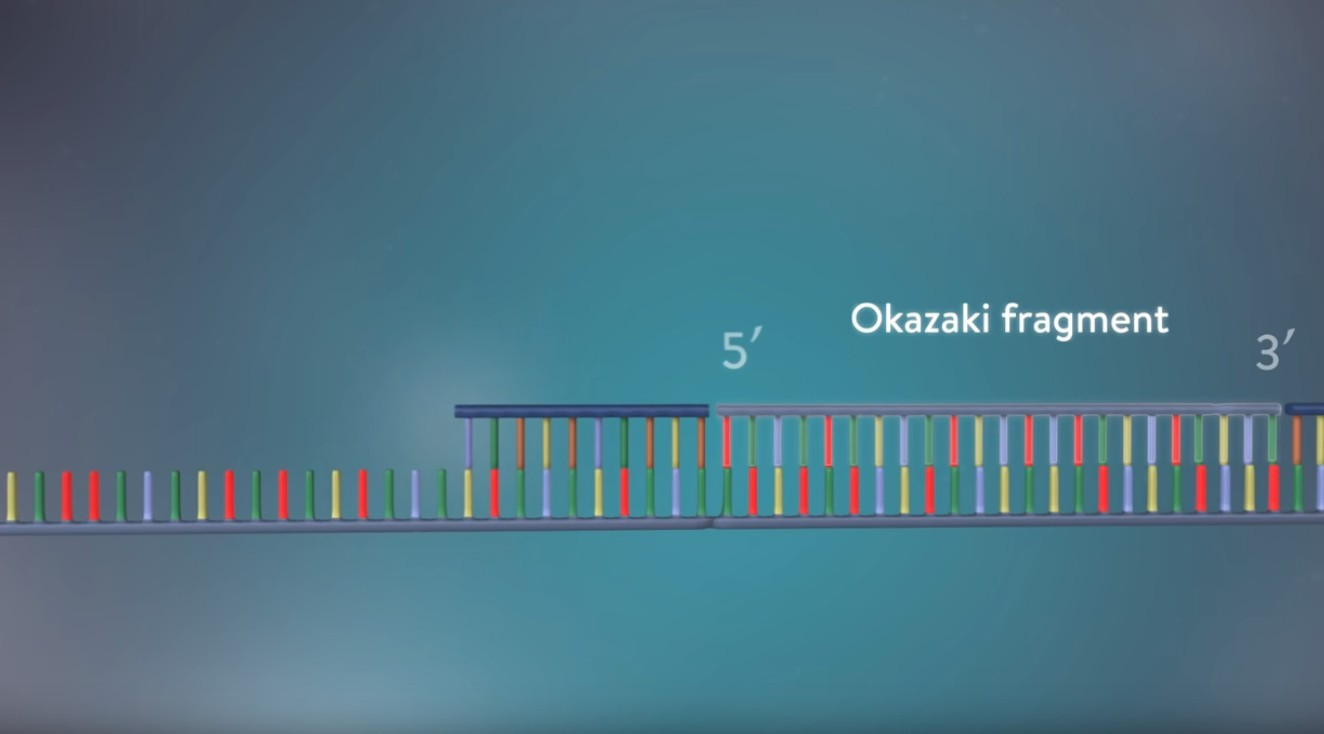
\includegraphics[width=\textwidth,height=0.6\textheight,keepaspectratio]{img/introduction/dna39.jpg}
		\label{img:mot2}
		\caption{In the lagging strand, the DNA polymerase can only make this strand in small chuncks (Okazaki fragment). }
	\end{figure}
\end{frame}
%-------------------------------------------------------
%-------------------------------------------------------

%-------------------------------------------------------
%-------------------------------------------------------
\begin{frame}{DNA replication}{Overview}
	\begin{figure}[]
		\centering
		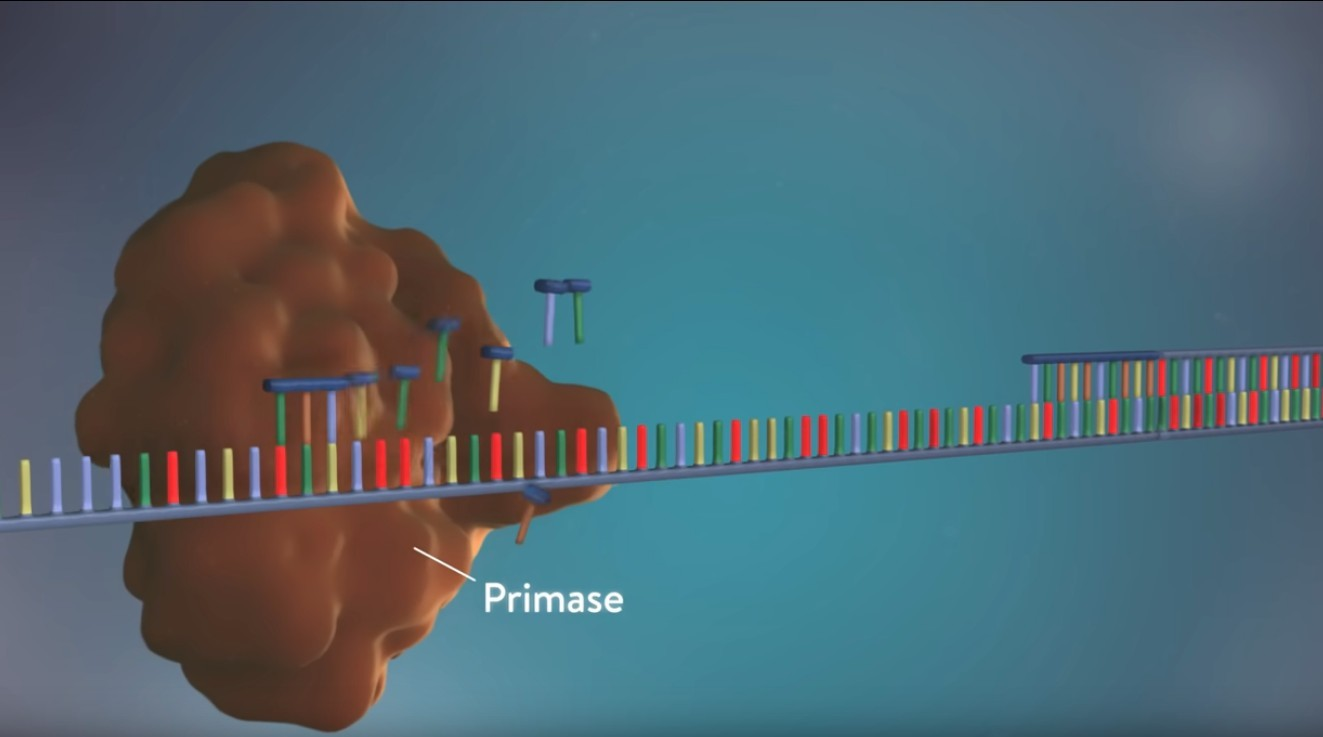
\includegraphics[width=\textwidth,height=0.6\textheight,keepaspectratio]{img/introduction/dna40.jpg}
		\label{img:mot2}
		\caption{In the lagging strand, each fragment is started with the enzyme Primase. }
	\end{figure}
\end{frame}
%-------------------------------------------------------
%-------------------------------------------------------

%-------------------------------------------------------
%-------------------------------------------------------
\begin{frame}{DNA replication}{Overview}
	\begin{figure}[]
		\centering
		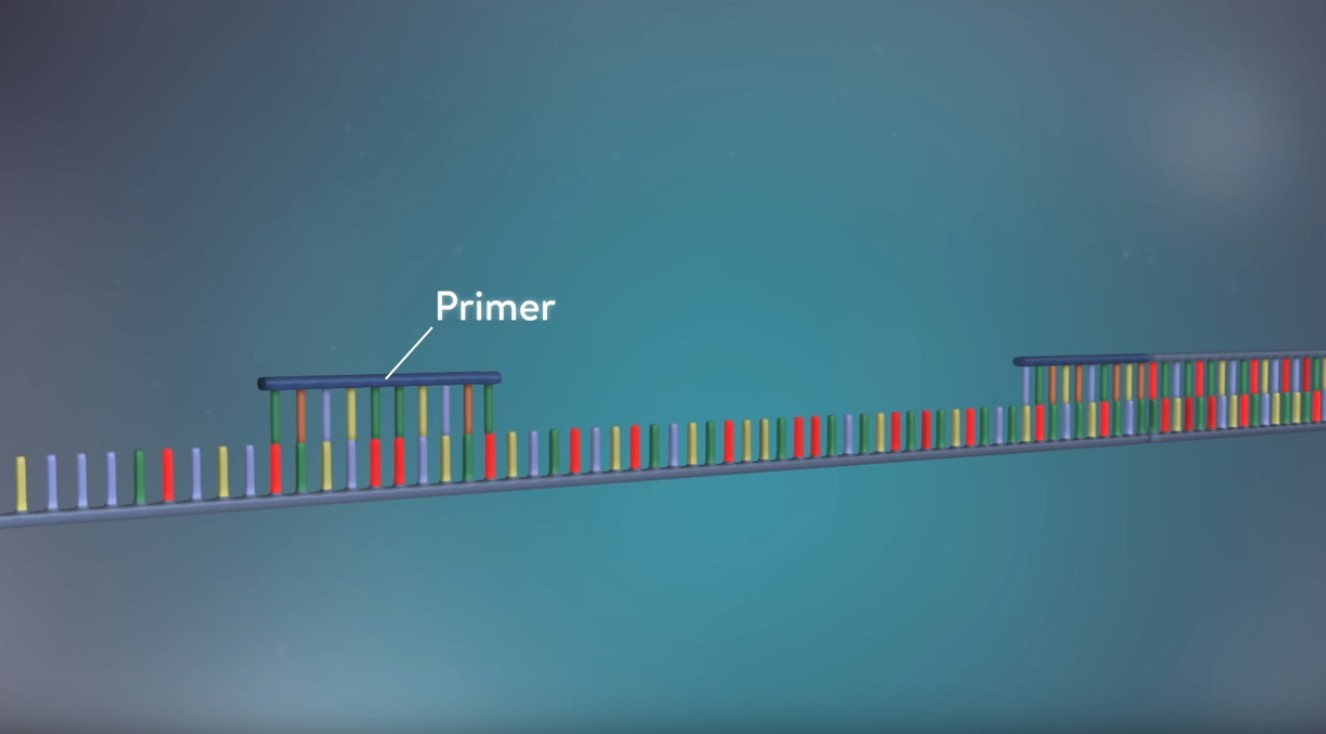
\includegraphics[width=\textwidth,height=0.6\textheight,keepaspectratio]{img/introduction/dna41.jpg}
		\label{img:mot2}
		\caption{In the lagging strand, the Primase insert the primer. }
	\end{figure}
\end{frame}
%-------------------------------------------------------
%-------------------------------------------------------


%-------------------------------------------------------
%-------------------------------------------------------
\begin{frame}{DNA replication}{Overview}
	\begin{figure}[]
		\centering
		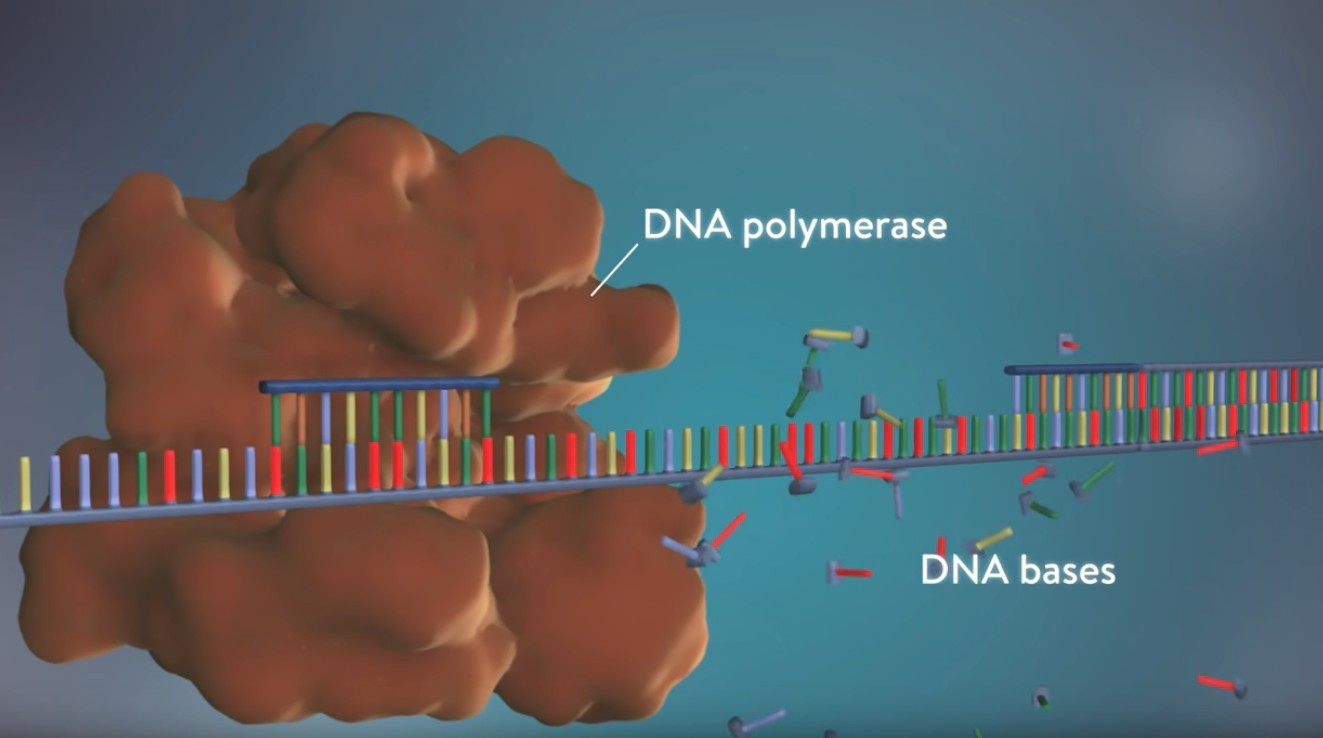
\includegraphics[width=\textwidth,height=0.6\textheight,keepaspectratio]{img/introduction/dna42.jpg}
		\label{img:mot2}
		\caption{The DNA polymerase add the DNA bases from 5' to 3' direction. }
	\end{figure}
\end{frame}
%-------------------------------------------------------
%-------------------------------------------------------

%-------------------------------------------------------
%-------------------------------------------------------
\begin{frame}{DNA replication}{Overview}
	\begin{figure}[]
		\centering
		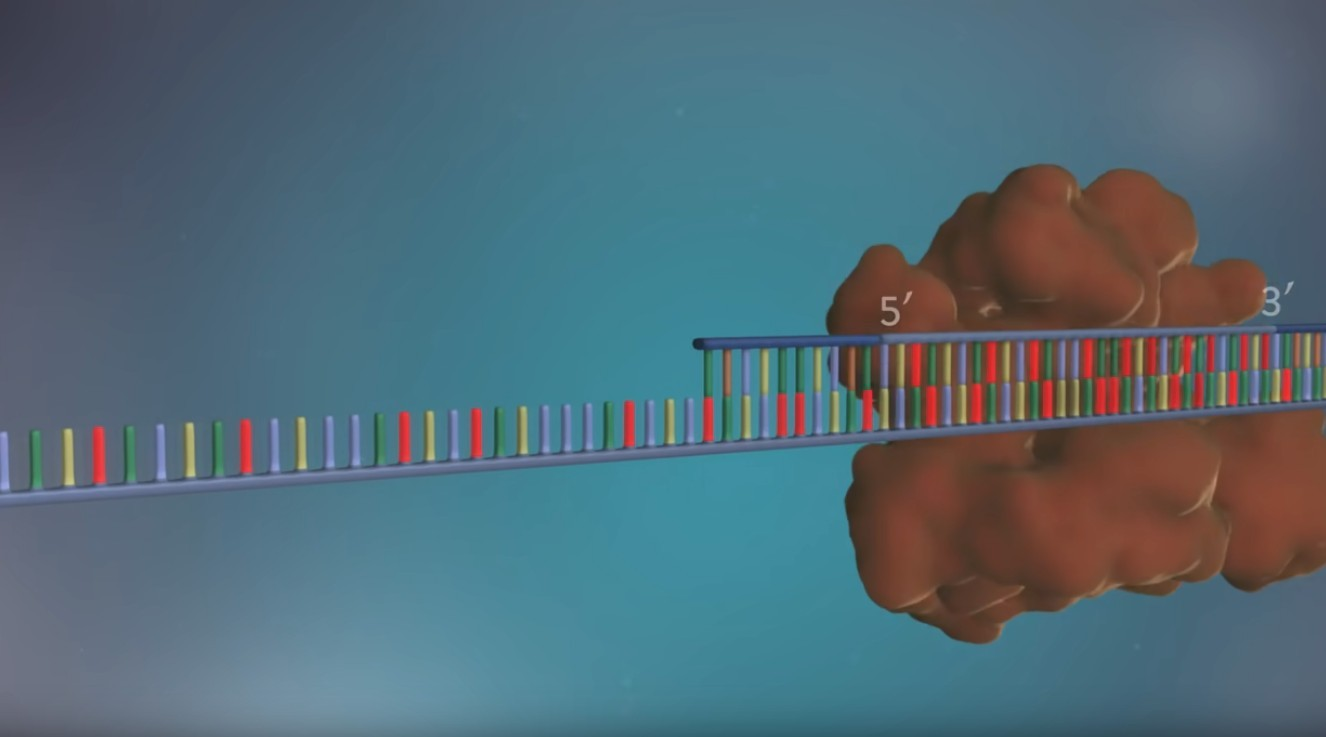
\includegraphics[width=\textwidth,height=0.6\textheight,keepaspectratio]{img/introduction/dna43.jpg}
		\label{img:mot2}
		\caption{The DNA polymerase add the DNA bases from 5' to 3' direction. }
	\end{figure}
\end{frame}
%-------------------------------------------------------
%-------------------------------------------------------


%-------------------------------------------------------
%-------------------------------------------------------
\begin{frame}{DNA replication}{Overview}
	\begin{figure}[]
		\centering
		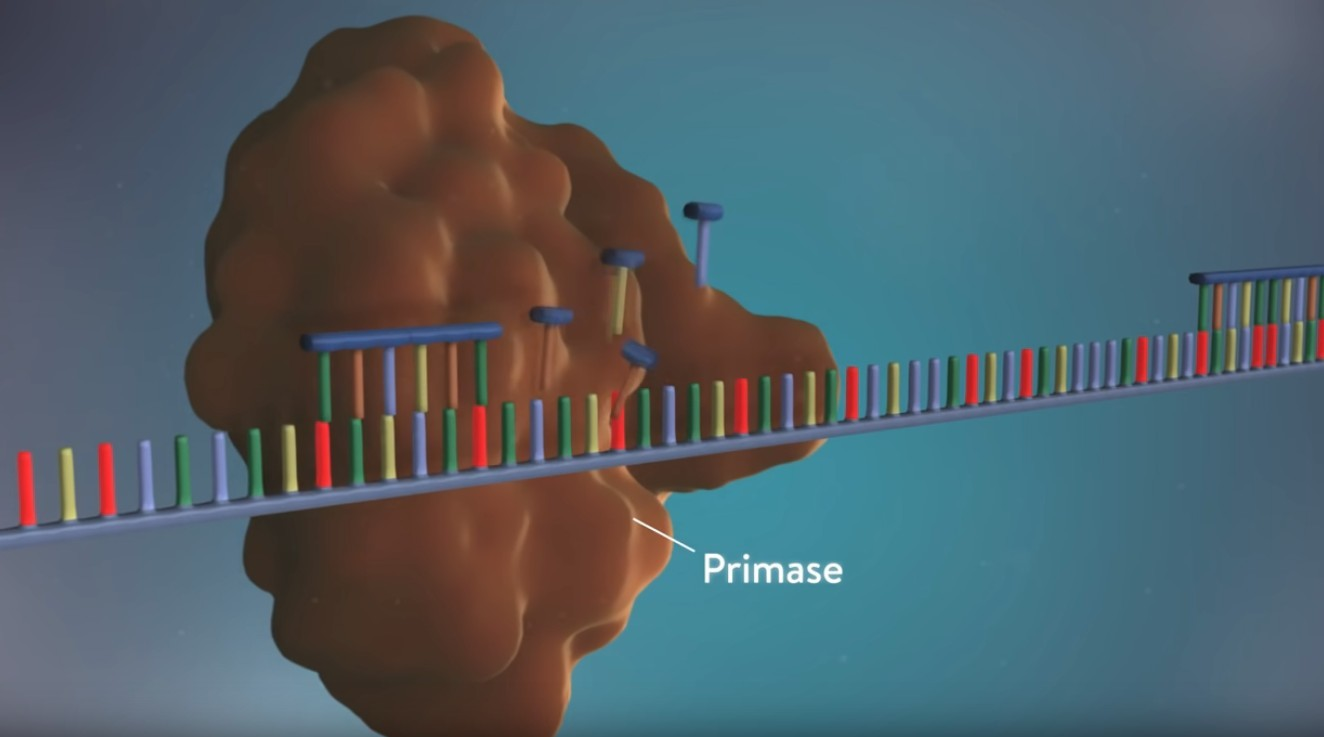
\includegraphics[width=\textwidth,height=0.6\textheight,keepaspectratio]{img/introduction/dna44.jpg}
		\label{img:mot2}
		\caption{The primer is added further down the lagging strand. }
	\end{figure}
\end{frame}
%-------------------------------------------------------
%-------------------------------------------------------

%-------------------------------------------------------
%-------------------------------------------------------
\begin{frame}{DNA replication}{Overview}
	\begin{figure}[]
		\centering
		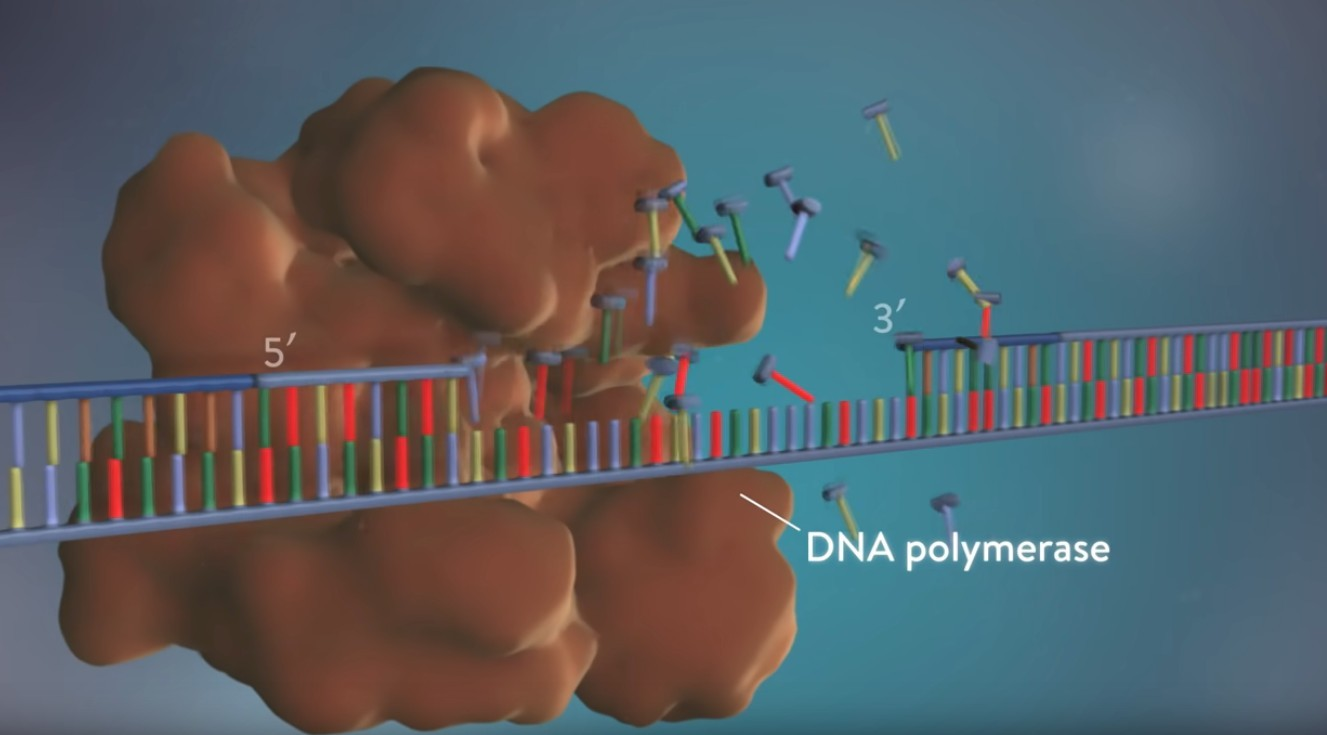
\includegraphics[width=\textwidth,height=0.6\textheight,keepaspectratio]{img/introduction/dna45.jpg}
		\label{img:mot2}
		\caption{Another Okazaki fragment is then made and the process is repeated again. }
	\end{figure}
\end{frame}
%-------------------------------------------------------
%-------------------------------------------------------


%-------------------------------------------------------
%-------------------------------------------------------
\begin{frame}{DNA replication}{Overview}
	\begin{figure}[]
		\centering
		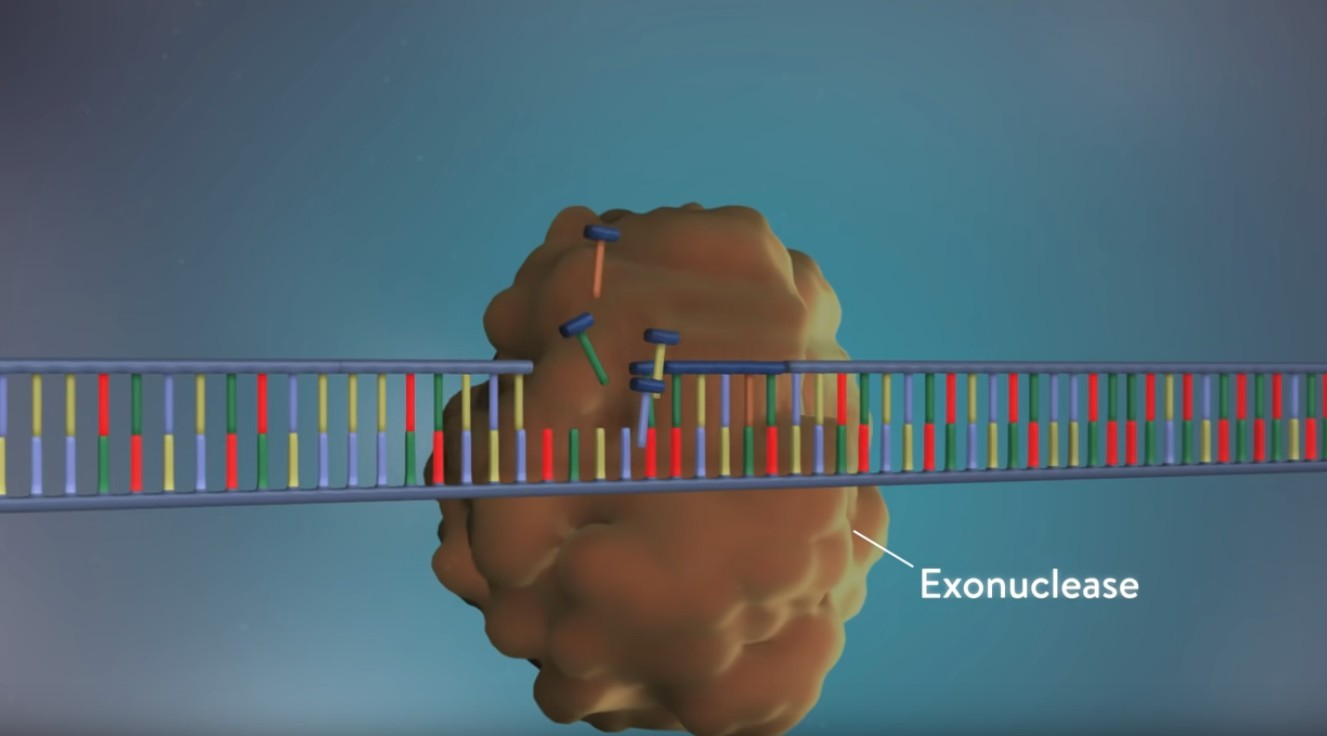
\includegraphics[width=\textwidth,height=0.6\textheight,keepaspectratio]{img/introduction/dna46.jpg}
		\label{img:mot2}
		\caption{Once the DNA has been made, the enzyme \textbf{Exonuclease} removes all the RNA primers from both strands of DNA }
	\end{figure}
\end{frame}
%-------------------------------------------------------
%-------------------------------------------------------

%-------------------------------------------------------
%-------------------------------------------------------
\begin{frame}{DNA replication}{Overview}
	\begin{figure}[]
		\centering
		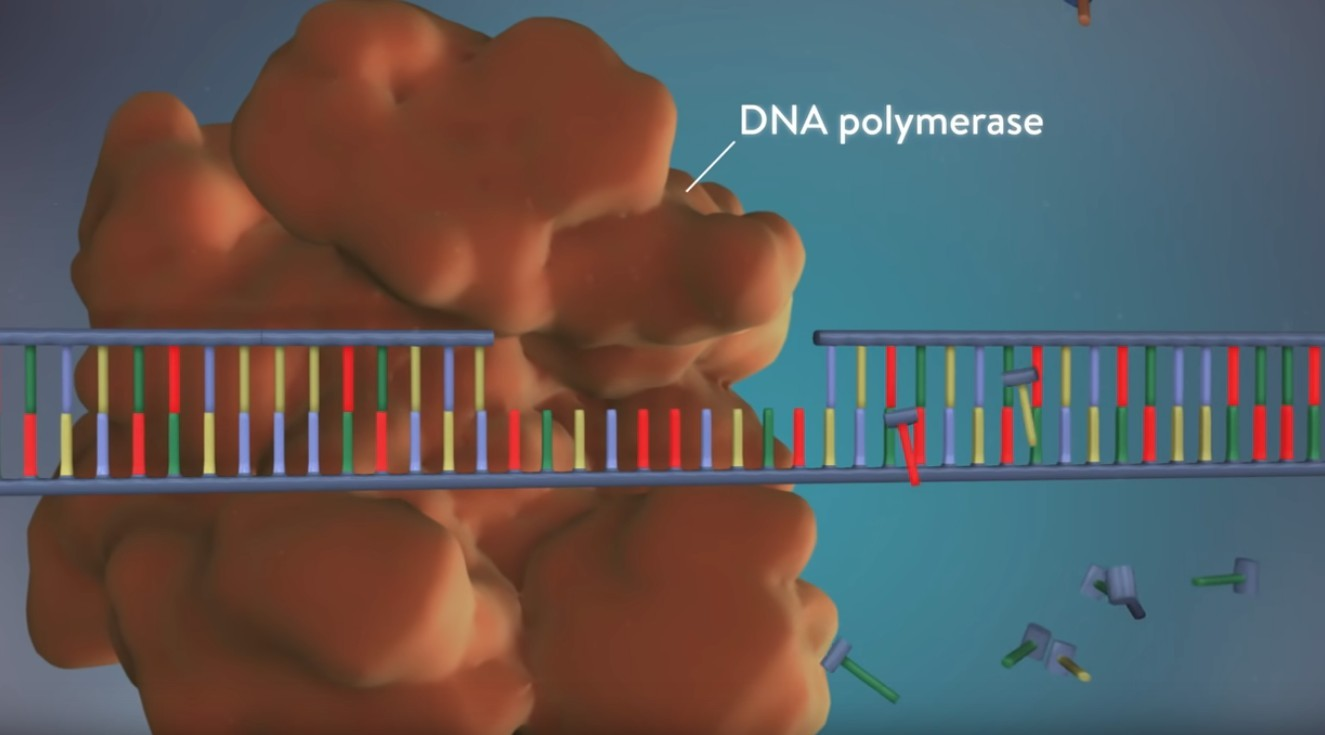
\includegraphics[width=\textwidth,height=0.6\textheight,keepaspectratio]{img/introduction/dna47.jpg}
		\label{img:mot2}
		\caption{Another DNA polymerase enzyme then fills in the gaps.}
	\end{figure}
\end{frame}
%-------------------------------------------------------
%-------------------------------------------------------


%-------------------------------------------------------
%-------------------------------------------------------
\begin{frame}{DNA replication}{Overview}
	\begin{figure}[]
		\centering
		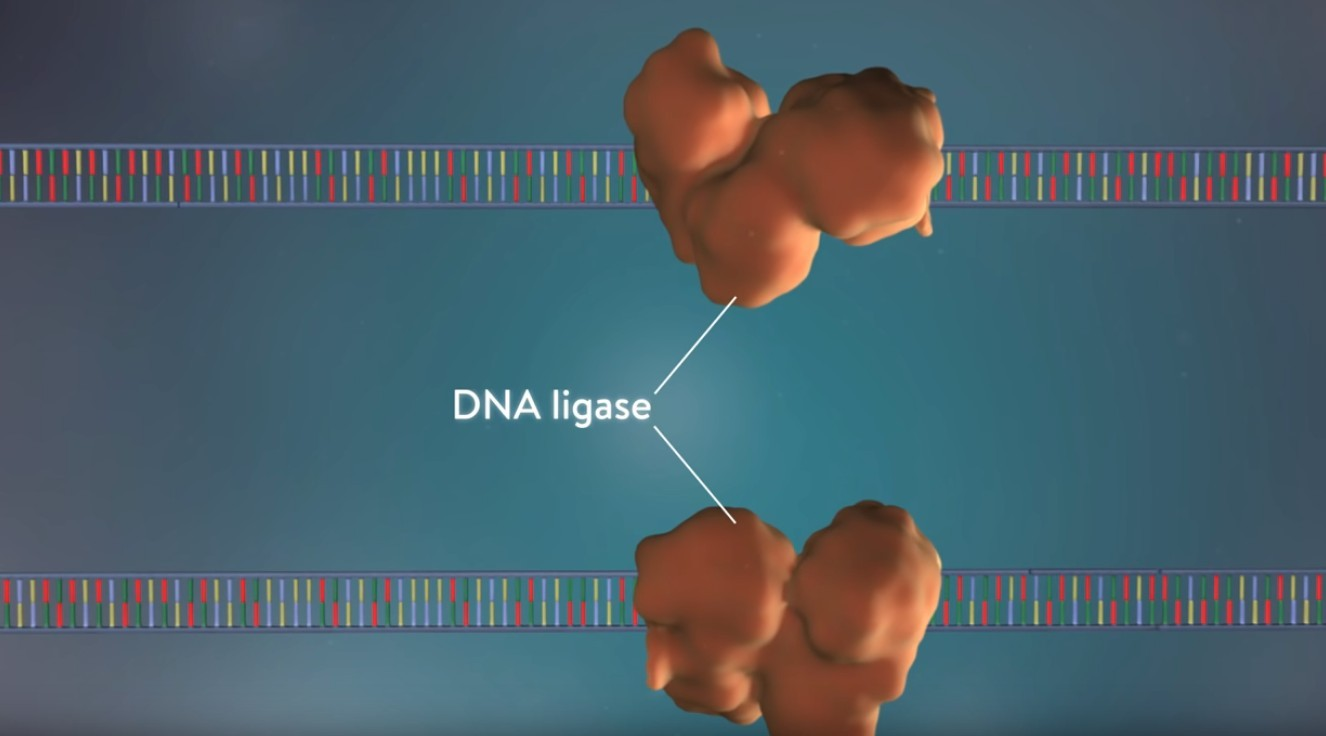
\includegraphics[width=\textwidth,height=0.6\textheight,keepaspectratio]{img/introduction/dna48.jpg}
		\label{img:mot2}
		\caption{Finally the enzyme \textbf{DNA ligase} seals up the fragments of DNA.}
	\end{figure}
\end{frame}
%-------------------------------------------------------
%-------------------------------------------------------

%-------------------------------------------------------
%-------------------------------------------------------
\begin{frame}{DNA replication}{Overview}
	\begin{figure}[]
		\centering
		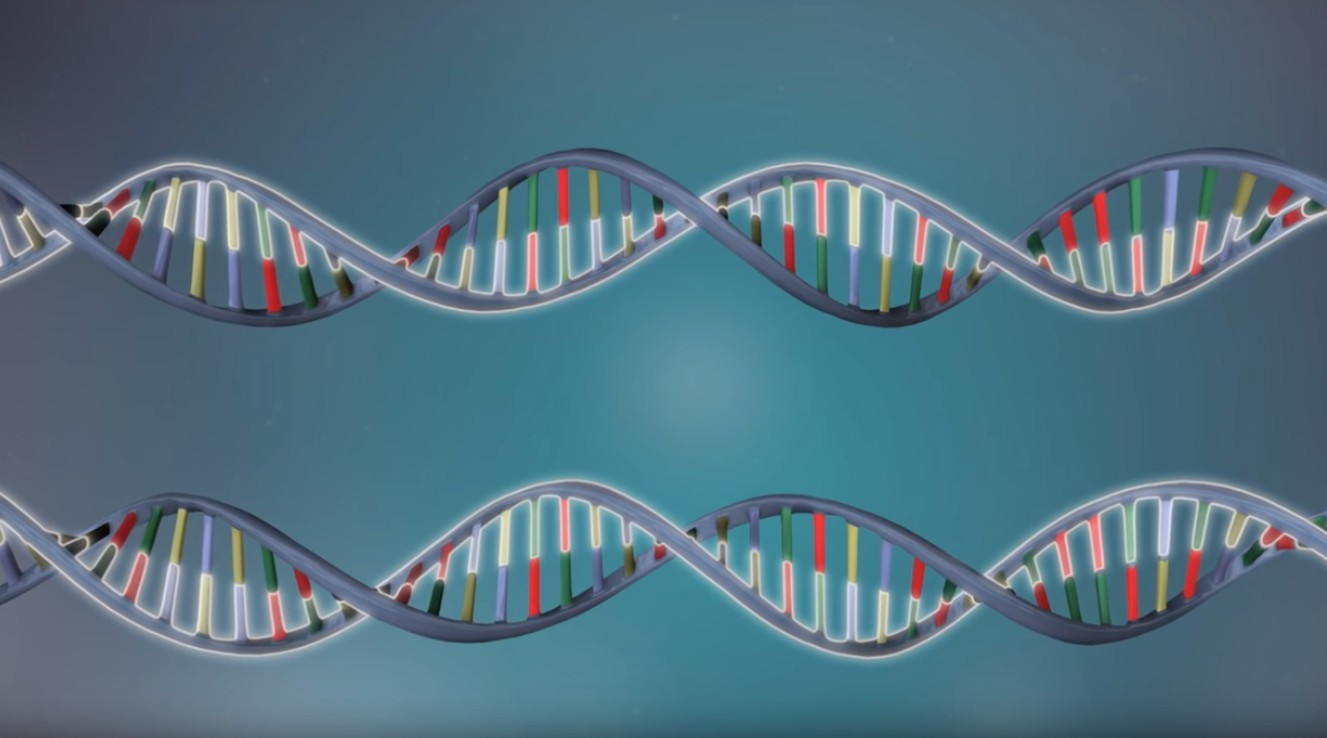
\includegraphics[width=\textwidth,height=0.6\textheight,keepaspectratio]{img/introduction/dna49.jpg}
		\label{img:mot2}
		\caption{DNA replication is describe as semi-conservative because each DNA molecule is made up from one old, conserved strand of DNA and one new.}
	\end{figure}
\end{frame}
%-------------------------------------------------------
%-------------------------------------------------------


%-------------------------------------------------------
%-------------------------------------------------------
\begin{frame}[allowframebreaks]
        \frametitle{References}
        %\bibliographystyle{amsalpha}
        \bibliographystyle{IEEEtran}
        \bibliography{bibliography.bib}
\end{frame}
%-------------------------------------------------------
%-------------------------------------------------------

%-------------------------------------------------------
%-------------------------------------------------------
\if\mycmd1 % MY THEME
\1{
	{\1
		\begin{frame}[plain,noframenumbering]
			\finalpage{Thank you}
		\end{frame}}
		\else % CS THEME
		
\fi
%-------------------------------------------------------
%-------------------------------------------------------



\end{document}